% !TeX program = pdflatex
% !TeX root = FCLoopGraphPlot.tex

\documentclass[../FeynCalcManual.tex]{subfiles}
\begin{document}
\hypertarget{fcloopgraphplot}{%
\section{FCLoopGraphPlot}\label{fcloopgraphplot}}

\texttt{FCLoopGraphPlot[\allowbreak{}\{\allowbreak{}edges,\ \allowbreak{}labels\}]}
visualizes the graph of the given loop integral using the provided list
of edges, styles and labels using the built-in function \texttt{Graph}.
The Option \texttt{Graph} can be used to pass options to the
\texttt{Graph} objects.

By default, \texttt{FCLoopGraphPlot} returns a \texttt{Graph}. When
using Mathematica 12.2 or newer, it is also possible to return a
\texttt{Graphics} object created by \texttt{GraphPlot}. For this the
option \texttt{GraphPlot} must be set to a list of options that will be
passed to \texttt{GraphPlot}. An empty list is also admissible. For
example,
\texttt{FCLoopGraphPlot[\allowbreak{}int,\ \allowbreak{}GraphPlot -> \{\allowbreak{}MultiedgeStyle -> 0.35,\ \allowbreak{}Frame -> True\}]}.

Given a list of \texttt{Graph} or \texttt{Graphics} objects created by
\texttt{FCLoopGraphPlot}, a nice way to get a better overview is to
employ
\texttt{Magnify[\allowbreak{}Grid[\allowbreak{}(Partition[\allowbreak{}out,\ \allowbreak{}UpTo[\allowbreak{}4]])],\ \allowbreak{}0.9]}.

Notice that older Mathematica versions have numerous shortcomings in the
graph drawing capabilities that cannot be reliably worked around. This
why to use \texttt{FCLoopGraphPlot} you need to have at least
Mathematica 11.0 or newer. For best results we recommend using
Mathematica 12.2 or newer.

\subsection{See also}

\hyperlink{toc}{Overview},
\hyperlink{fcloopintegraltograph}{FCLoopIntegralToGraph}.

\subsection{Examples}

\hypertarget{showcases}\OperatorTok{]}
\end{Highlighting}
\end{Shaded}

\begin{dmath*}\breakingcomma
\left\{\{1\to 1\},\left(
\begin{array}{ccc}
 p & 1 & -m^2 \\
\end{array}
\right),\left\{\frac{1}{(p^2-m^2+i \eta )}\right\},1\right\}
\end{dmath*}

\begin{figure}[!ht]
\centering
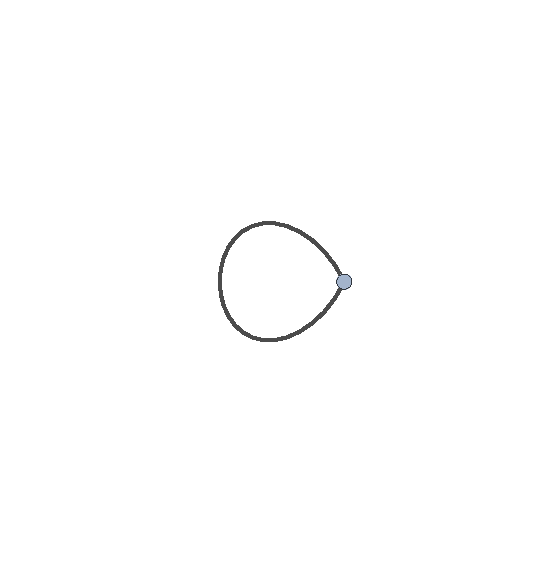
\includegraphics[width=0.6\linewidth]{img/0yvbg69o85nqi.pdf}
\end{figure}

1-loop massless bubble

\begin{Shaded}
\begin{Highlighting}[]
\NormalTok{FCLoopIntegralToGraph}\OperatorTok{[}\NormalTok{FAD}\OperatorTok{[}\FunctionTok{p}\OperatorTok{,} \FunctionTok{p} \SpecialCharTok{{-}} \FunctionTok{q}\OperatorTok{],} \OperatorTok{\{}\FunctionTok{p}\OperatorTok{\}]} 
 
\NormalTok{FCLoopGraphPlot}\OperatorTok{[}\SpecialCharTok{\%}\OperatorTok{]}
\end{Highlighting}
\end{Shaded}

\begin{dmath*}\breakingcomma
\left\{\{-3\to 2,-1\to 1,1\to 2,1\to 2\},\{q,q,\{p,1,0\},\{p-q,1,0\}\},\left\{0,0,\frac{1}{(p^2+i \eta )},\frac{1}{((p-q)^2+i \eta )}\right\},1\right\}
\end{dmath*}

\begin{figure}[!ht]
\centering
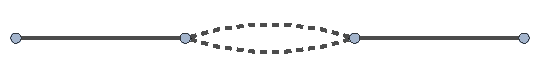
\includegraphics[width=0.6\linewidth]{img/18zlvfvc5dy6q.pdf}
\end{figure}

1-loop massive bubble

\begin{Shaded}
\begin{Highlighting}[]
\NormalTok{FCLoopIntegralToGraph}\OperatorTok{[}\NormalTok{FAD}\OperatorTok{[\{}\FunctionTok{p}\OperatorTok{,}\NormalTok{ m1}\OperatorTok{\},} \OperatorTok{\{}\FunctionTok{p} \SpecialCharTok{{-}} \FunctionTok{q}\OperatorTok{,}\NormalTok{ m2}\OperatorTok{\}],} \OperatorTok{\{}\FunctionTok{p}\OperatorTok{\}]} 
 
\NormalTok{FCLoopGraphPlot}\OperatorTok{[}\SpecialCharTok{\%}\OperatorTok{]}
\end{Highlighting}
\end{Shaded}

\begin{dmath*}\breakingcomma
\left\{\{-3\to 2,-1\to 1,1\to 2,1\to 2\},\left\{q,q,\left\{p,1,-\text{m1}^2\right\},\left\{p-q,1,-\text{m2}^2\right\}\right\},\left\{0,0,\frac{1}{(p^2-\text{m1}^2+i \eta )},\frac{1}{((p-q)^2-\text{m2}^2+i \eta )}\right\},1\right\}
\end{dmath*}

\begin{figure}[!ht]
\centering
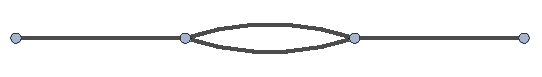
\includegraphics[width=0.6\linewidth]{img/0mx2npuji2kki.pdf}
\end{figure}

1-loop massless triangle

\begin{Shaded}
\begin{Highlighting}[]
\NormalTok{FCLoopIntegralToGraph}\OperatorTok{[}\NormalTok{FAD}\OperatorTok{[}\FunctionTok{p}\OperatorTok{,} \FunctionTok{p} \SpecialCharTok{+}\NormalTok{ q1}\OperatorTok{,} \FunctionTok{p} \SpecialCharTok{+}\NormalTok{ q1 }\SpecialCharTok{+}\NormalTok{ q2}\OperatorTok{],} \OperatorTok{\{}\FunctionTok{p}\OperatorTok{\}]} 
 
\NormalTok{FCLoopGraphPlot}\OperatorTok{[}\SpecialCharTok{\%}\OperatorTok{]}
\end{Highlighting}
\end{Shaded}

\begin{dmath*}\breakingcomma
\left\{\{-3\to 3,-2\to 1,-1\to 2,1\to 2,1\to 3,2\to 3\},\{\text{q1}-\text{q2},\text{q1},\text{q2},\{p+\text{q1},1,0\},\{p+\text{q1}+\text{q2},1,0\},\{p,1,0\}\},\left\{0,0,0,\frac{1}{(p^2+i \eta )},\frac{1}{((p+\text{q1})^2+i \eta )},\frac{1}{((p+\text{q1}+\text{q2})^2+i \eta )}\right\},1\right\}
\end{dmath*}

\begin{figure}[!ht]
\centering
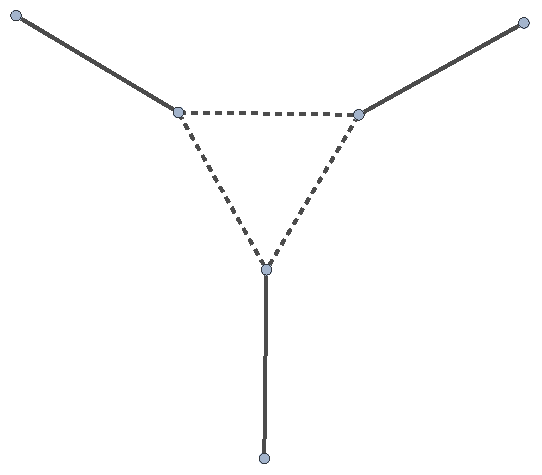
\includegraphics[width=0.6\linewidth]{img/1veisicnoyp27.pdf}
\end{figure}

1-loop massless box

\begin{Shaded}
\begin{Highlighting}[]
\NormalTok{FCLoopIntegralToGraph}\OperatorTok{[}\NormalTok{FAD}\OperatorTok{[}\FunctionTok{p}\OperatorTok{,} \FunctionTok{p} \SpecialCharTok{+}\NormalTok{ q1}\OperatorTok{,} \FunctionTok{p} \SpecialCharTok{+}\NormalTok{ q1 }\SpecialCharTok{+}\NormalTok{ q2}\OperatorTok{,} \FunctionTok{p} \SpecialCharTok{+}\NormalTok{ q1 }\SpecialCharTok{+}\NormalTok{ q2 }\SpecialCharTok{+}\NormalTok{ q3}\OperatorTok{],} \OperatorTok{\{}\FunctionTok{p}\OperatorTok{\}]} 
 
\NormalTok{FCLoopGraphPlot}\OperatorTok{[}\SpecialCharTok{\%}\OperatorTok{]}
\end{Highlighting}
\end{Shaded}

\begin{dmath*}\breakingcomma
\left\{\{-4\to 4,-3\to 1,-2\to 2,-1\to 3,1\to 2,1\to 4,2\to 3,3\to 4\},\{\text{q1}-\text{q2}-\text{q3},\text{q1},\text{q2},\text{q3},\{p+\text{q1}+\text{q2},1,0\},\{p+\text{q1}+\text{q2}+\text{q3},1,0\},\{p+\text{q1},1,0\},\{p,1,0\}\},\left\{0,0,0,0,\frac{1}{(p^2+i \eta )},\frac{1}{((p+\text{q1})^2+i \eta )},\frac{1}{((p+\text{q1}+\text{q2})^2+i \eta )},\frac{1}{((p+\text{q1}+\text{q2}+\text{q3})^2+i \eta )}\right\},1\right\}
\end{dmath*}

\begin{figure}[!ht]
\centering
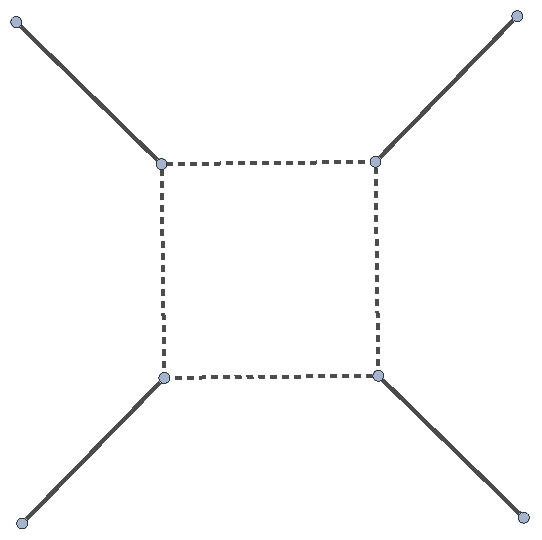
\includegraphics[width=0.6\linewidth]{img/0gnj7wff0851c.pdf}
\end{figure}

1-loop massless pentagon

\begin{Shaded}
\begin{Highlighting}[]
\NormalTok{FCLoopIntegralToGraph}\OperatorTok{[}\NormalTok{FAD}\OperatorTok{[}\FunctionTok{p}\OperatorTok{,} \FunctionTok{p} \SpecialCharTok{+}\NormalTok{ q1}\OperatorTok{,} \FunctionTok{p} \SpecialCharTok{+}\NormalTok{ q1 }\SpecialCharTok{+}\NormalTok{ q2}\OperatorTok{,} \FunctionTok{p} \SpecialCharTok{+}\NormalTok{ q1 }\SpecialCharTok{+}\NormalTok{ q2 }\SpecialCharTok{+}\NormalTok{ q3}\OperatorTok{,} \FunctionTok{p} \SpecialCharTok{+}\NormalTok{ q1 }\SpecialCharTok{+}\NormalTok{ q2 }\SpecialCharTok{+}\NormalTok{ q3 }\SpecialCharTok{+}\NormalTok{ q4}\OperatorTok{],} \OperatorTok{\{}\FunctionTok{p}\OperatorTok{\}]} 
 
\NormalTok{FCLoopGraphPlot}\OperatorTok{[}\SpecialCharTok{\%}\OperatorTok{]}
\end{Highlighting}
\end{Shaded}

\begin{dmath*}\breakingcomma
\left\{\{-5\to 5,-4\to 1,-3\to 2,-2\to 3,-1\to 4,1\to 2,1\to 5,2\to 3,3\to 4,4\to 5\},\{\text{q1}-\text{q2}-\text{q3}-\text{q4},\text{q1},\text{q2},\text{q3},\text{q4},\{p+\text{q1}+\text{q2}+\text{q3},1,0\},\{p+\text{q1}+\text{q2}+\text{q3}+\text{q4},1,0\},\{p+\text{q1}+\text{q2},1,0\},\{p+\text{q1},1,0\},\{p,1,0\}\},\left\{0,0,0,0,0,\frac{1}{(p^2+i \eta )},\frac{1}{((p+\text{q1})^2+i \eta )},\frac{1}{((p+\text{q1}+\text{q2})^2+i \eta )},\frac{1}{((p+\text{q1}+\text{q2}+\text{q3})^2+i \eta )},\frac{1}{((p+\text{q1}+\text{q2}+\text{q3}+\text{q4})^2+i \eta )}\right\},1\right\}
\end{dmath*}

\begin{figure}[!ht]
\centering
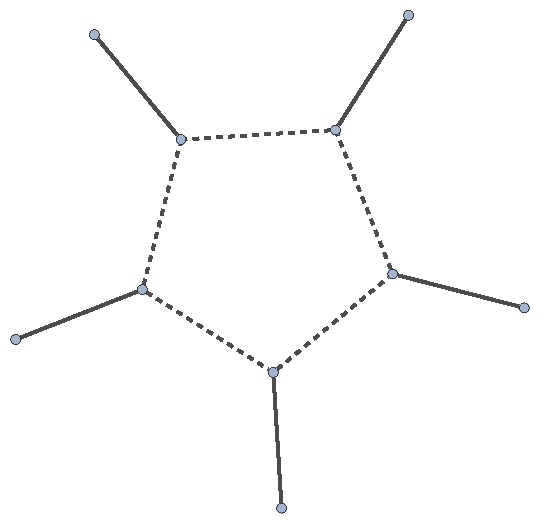
\includegraphics[width=0.6\linewidth]{img/0w423j5lcoh4g.pdf}
\end{figure}

2-loop massless self-energy

\begin{Shaded}
\begin{Highlighting}[]
\NormalTok{FCLoopIntegralToGraph}\OperatorTok{[}\NormalTok{FAD}\OperatorTok{[}\NormalTok{p1}\OperatorTok{,}\NormalTok{ p2}\OperatorTok{,} \FunctionTok{Q} \SpecialCharTok{{-}}\NormalTok{ p1 }\SpecialCharTok{{-}}\NormalTok{ p2}\OperatorTok{,} \FunctionTok{Q} \SpecialCharTok{{-}}\NormalTok{ p1}\OperatorTok{,} \FunctionTok{Q} \SpecialCharTok{{-}}\NormalTok{ p2}\OperatorTok{],} \OperatorTok{\{}\NormalTok{p1}\OperatorTok{,}\NormalTok{ p2}\OperatorTok{\}]} 
 
\NormalTok{FCLoopGraphPlot}\OperatorTok{[}\SpecialCharTok{\%}\OperatorTok{]}
\end{Highlighting}
\end{Shaded}

\begin{dmath*}\breakingcomma
\left\{\{-3\to 2,-1\to 1,1\to 3,1\to 4,2\to 3,2\to 4,3\to 4\},\{Q,Q,\{\text{p2},1,0\},\{Q-\text{p2},1,0\},\{Q-\text{p1},1,0\},\{\text{p1},1,0\},\{-\text{p1}-\text{p2}+Q,1,0\}\},\left\{0,0,\frac{1}{(\text{p2}^2+i \eta )},\frac{1}{(\text{p1}^2+i \eta )},\frac{1}{((Q-\text{p2})^2+i \eta )},\frac{1}{((Q-\text{p1})^2+i \eta )},\frac{1}{((-\text{p1}-\text{p2}+Q)^2+i \eta )}\right\},1\right\}
\end{dmath*}

\begin{figure}[!ht]
\centering
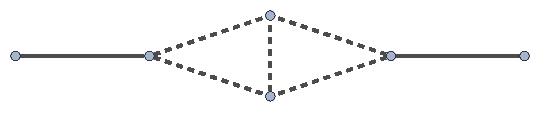
\includegraphics[width=0.6\linewidth]{img/0m09banu3jlo2.pdf}
\end{figure}

Same topology as before but now fully massive and with some dots

\begin{Shaded}
\begin{Highlighting}[]
\NormalTok{FCLoopIntegralToGraph}\OperatorTok{[}\NormalTok{FAD}\OperatorTok{[\{}\NormalTok{p1}\OperatorTok{,} \FunctionTok{m}\OperatorTok{\},} \OperatorTok{\{}\NormalTok{p2}\OperatorTok{,}\NormalTok{ m2}\OperatorTok{\},} \OperatorTok{\{}\FunctionTok{Q} \SpecialCharTok{{-}}\NormalTok{ p1 }\SpecialCharTok{{-}}\NormalTok{ p2}\OperatorTok{,} \FunctionTok{m}\OperatorTok{\},} \OperatorTok{\{}\FunctionTok{Q} \SpecialCharTok{{-}}\NormalTok{ p1}\OperatorTok{,} \FunctionTok{m}\OperatorTok{,} \DecValTok{2}\OperatorTok{\},} \OperatorTok{\{}\FunctionTok{Q} \SpecialCharTok{{-}}\NormalTok{ p2}\OperatorTok{,} \FunctionTok{m}\OperatorTok{,}\DecValTok{2}\OperatorTok{\}],} \OperatorTok{\{}\NormalTok{p1}\OperatorTok{,}\NormalTok{ p2}\OperatorTok{\}]} 
 
\NormalTok{FCLoopGraphPlot}\OperatorTok{[}\SpecialCharTok{\%}\OperatorTok{]}
\end{Highlighting}
\end{Shaded}

\begin{dmath*}\breakingcomma
\left\{\{-3\to 2,-1\to 1,1\to 3,1\to 4,2\to 3,2\to 4,3\to 4\},\left\{Q,Q,\left\{\text{p2},1,-\text{m2}^2\right\},\left\{Q-\text{p2},2,-m^2\right\},\left\{Q-\text{p1},2,-m^2\right\},\left\{\text{p1},1,-m^2\right\},\left\{-\text{p1}-\text{p2}+Q,1,-m^2\right\}\right\},\left\{0,0,\frac{1}{(\text{p2}^2-\text{m2}^2+i \eta )},\frac{1}{(\text{p1}^2-m^2+i \eta )},\frac{1}{((Q-\text{p2})^2-m^2+i \eta )},\frac{1}{((Q-\text{p1})^2-m^2+i \eta )},\frac{1}{((-\text{p1}-\text{p2}+Q)^2-m^2+i \eta )}\right\},1\right\}
\end{dmath*}

\begin{figure}[!ht]
\centering
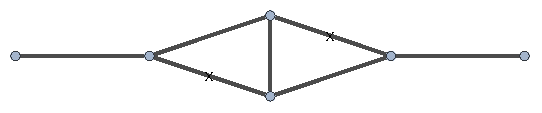
\includegraphics[width=0.6\linewidth]{img/0p4vf5g6fykzy.pdf}
\end{figure}

3-loop massless self-energy

\begin{Shaded}
\begin{Highlighting}[]
\NormalTok{FCLoopIntegralToGraph}\OperatorTok{[}\NormalTok{FAD}\OperatorTok{[}\NormalTok{p1}\OperatorTok{,}\NormalTok{ p2}\OperatorTok{,}\NormalTok{ p3}\OperatorTok{,} \FunctionTok{Q} \SpecialCharTok{{-}}\NormalTok{ p1 }\SpecialCharTok{{-}}\NormalTok{ p2 }\SpecialCharTok{{-}}\NormalTok{ p3}\OperatorTok{,} \FunctionTok{Q} \SpecialCharTok{{-}}\NormalTok{ p1 }\SpecialCharTok{{-}}\NormalTok{ p2}\OperatorTok{,} \FunctionTok{Q} \SpecialCharTok{{-}}\NormalTok{ p1}\OperatorTok{,} \FunctionTok{Q} \SpecialCharTok{{-}}\NormalTok{ p2}\OperatorTok{,}\NormalTok{ p1 }\SpecialCharTok{+}\NormalTok{ p3}\OperatorTok{],} \OperatorTok{\{}\NormalTok{p1}\OperatorTok{,}\NormalTok{ p2}\OperatorTok{,}\NormalTok{ p3}\OperatorTok{\}]} 
 
\NormalTok{FCLoopGraphPlot}\OperatorTok{[}\SpecialCharTok{\%}\OperatorTok{]}
\end{Highlighting}
\end{Shaded}

\begin{dmath*}\breakingcomma
\left\{\{-3\to 2,-1\to 1,1\to 5,1\to 6,2\to 3,2\to 5,3\to 4,3\to 6,4\to 5,4\to 6\},\{Q,Q,\{\text{p2},1,0\},\{Q-\text{p2},1,0\},\{\text{p1},1,0\},\{Q-\text{p1},1,0\},\{\text{p3},1,0\},\{\text{p1}+\text{p3},1,0\},\{-\text{p1}-\text{p2}+Q,1,0\},\{-\text{p1}-\text{p2}-\text{p3}+Q,1,0\}\},\left\{0,0,\frac{1}{(\text{p3}^2+i \eta )},\frac{1}{(\text{p2}^2+i \eta )},\frac{1}{(\text{p1}^2+i \eta )},\frac{1}{((\text{p1}+\text{p3})^2+i \eta )},\frac{1}{((Q-\text{p2})^2+i \eta )},\frac{1}{((Q-\text{p1})^2+i \eta )},\frac{1}{((-\text{p1}-\text{p2}+Q)^2+i \eta )},\frac{1}{((-\text{p1}-\text{p2}-\text{p3}+Q)^2+i \eta )}\right\},1\right\}
\end{dmath*}

\begin{figure}[!ht]
\centering
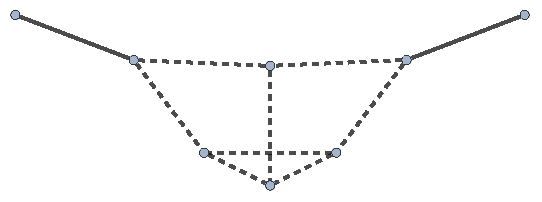
\includegraphics[width=0.6\linewidth]{img/177i8h9zggmck.pdf}
\end{figure}

3-loop self-energy with two massive lines

\begin{Shaded}
\begin{Highlighting}[]
\NormalTok{FCLoopIntegralToGraph}\OperatorTok{[}\FunctionTok{Times}\NormalTok{ @@ }\OperatorTok{\{}\NormalTok{SFAD}\OperatorTok{[\{\{}\NormalTok{p1}\OperatorTok{,} \DecValTok{0}\OperatorTok{\},} \OperatorTok{\{}\FunctionTok{m}\SpecialCharTok{\^{}}\DecValTok{2}\OperatorTok{,} \DecValTok{1}\OperatorTok{\},} \DecValTok{1}\OperatorTok{\}],}\NormalTok{ SFAD}\OperatorTok{[\{\{}\NormalTok{p2}\OperatorTok{,} \DecValTok{0}\OperatorTok{\},} \OperatorTok{\{}\DecValTok{0}\OperatorTok{,} \DecValTok{1}\OperatorTok{\},} \DecValTok{1}\OperatorTok{\}],} 
\NormalTok{     SFAD}\OperatorTok{[\{\{}\NormalTok{p3}\OperatorTok{,} \DecValTok{0}\OperatorTok{\},} \OperatorTok{\{}\DecValTok{0}\OperatorTok{,} \DecValTok{1}\OperatorTok{\},} \DecValTok{1}\OperatorTok{\}],}\NormalTok{ SFAD}\OperatorTok{[\{\{}\NormalTok{p1 }\SpecialCharTok{+}\NormalTok{ p2 }\SpecialCharTok{+}\NormalTok{ p3 }\SpecialCharTok{{-}} \FunctionTok{Q}\OperatorTok{,} \DecValTok{0}\OperatorTok{\},} \OperatorTok{\{}\DecValTok{0}\OperatorTok{,} \DecValTok{1}\OperatorTok{\},} \DecValTok{1}\OperatorTok{\}],}\NormalTok{ SFAD}\OperatorTok{[\{\{}\NormalTok{p2 }\SpecialCharTok{+}\NormalTok{ p3}\OperatorTok{,} \DecValTok{0}\OperatorTok{\},} \OperatorTok{\{}\DecValTok{0}\OperatorTok{,} \DecValTok{1}\OperatorTok{\},} \DecValTok{1}\OperatorTok{\}],} 
\NormalTok{     SFAD}\OperatorTok{[\{\{}\NormalTok{p2 }\SpecialCharTok{{-}} \FunctionTok{Q}\OperatorTok{,} \DecValTok{0}\OperatorTok{\},} \OperatorTok{\{}\DecValTok{0}\OperatorTok{,} \DecValTok{1}\OperatorTok{\},} \DecValTok{1}\OperatorTok{\}],}\NormalTok{ SFAD}\OperatorTok{[\{\{}\NormalTok{p1 }\SpecialCharTok{{-}} \FunctionTok{Q}\OperatorTok{,} \DecValTok{0}\OperatorTok{\},} \OperatorTok{\{}\FunctionTok{m}\SpecialCharTok{\^{}}\DecValTok{2}\OperatorTok{,} \DecValTok{1}\OperatorTok{\},} \DecValTok{1}\OperatorTok{\}],}\NormalTok{SFAD}\OperatorTok{[\{\{}\NormalTok{p2 }\SpecialCharTok{+}\NormalTok{ p3 }\SpecialCharTok{{-}} \FunctionTok{Q}\OperatorTok{,} \DecValTok{0}\OperatorTok{\},} \OperatorTok{\{}\DecValTok{0}\OperatorTok{,} \DecValTok{1}\OperatorTok{\},} \DecValTok{1}\OperatorTok{\}]\},} 
   \OperatorTok{\{}\NormalTok{p1}\OperatorTok{,}\NormalTok{ p2}\OperatorTok{,}\NormalTok{ p3}\OperatorTok{\}]} 
 
\NormalTok{FCLoopGraphPlot}\OperatorTok{[}\SpecialCharTok{\%}\OperatorTok{]}
\end{Highlighting}
\end{Shaded}

\begin{dmath*}\breakingcomma
\left\{\{-3\to 2,-1\to 1,1\to 3,1\to 4,2\to 5,2\to 6,3\to 4,3\to 5,4\to 6,5\to 6\},\left\{Q,Q,\{\text{p2},1,0\},\{\text{p2}-Q,1,0\},\left\{\text{p1}-Q,1,-m^2\right\},\left\{\text{p1},1,-m^2\right\},\{\text{p3},1,0\},\{\text{p2}+\text{p3},1,0\},\{\text{p2}+\text{p3}-Q,1,0\},\{\text{p1}+\text{p2}+\text{p3}-Q,1,0\}\right\},\left\{0,0,\frac{1}{(\text{p3}^2+i \eta )},\frac{1}{(\text{p2}^2+i \eta )},\frac{1}{((\text{p2}+\text{p3})^2+i \eta )},\frac{1}{((\text{p2}-Q)^2+i \eta )},\frac{1}{(\text{p1}^2-m^2+i \eta )},\frac{1}{((\text{p2}+\text{p3}-Q)^2+i \eta )},\frac{1}{((\text{p1}+\text{p2}+\text{p3}-Q)^2+i \eta )},\frac{1}{((\text{p1}-Q)^2-m^2+i \eta )}\right\},1\right\}
\end{dmath*}

\begin{figure}[!ht]
\centering
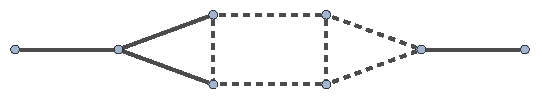
\includegraphics[width=0.6\linewidth]{img/0epatn35bxucj.pdf}
\end{figure}

2-loop triangle

\begin{Shaded}
\begin{Highlighting}[]
\NormalTok{FCLoopIntegralToGraph}\OperatorTok{[}\NormalTok{FAD}\OperatorTok{[}\NormalTok{p1}\OperatorTok{,}\NormalTok{ p2}\OperatorTok{,}\NormalTok{ Q1 }\SpecialCharTok{+}\NormalTok{ p1}\OperatorTok{,}\NormalTok{ Q2 }\SpecialCharTok{{-}}\NormalTok{ p1}\OperatorTok{,}\NormalTok{ Q1 }\SpecialCharTok{+}\NormalTok{ p1 }\SpecialCharTok{+}\NormalTok{ p2}\OperatorTok{,}\NormalTok{ Q2 }\SpecialCharTok{{-}}\NormalTok{ p1 }\SpecialCharTok{{-}}\NormalTok{ p2}\OperatorTok{],} \OperatorTok{\{}\NormalTok{p1}\OperatorTok{,}\NormalTok{ p2}\OperatorTok{\}]} 
 
\NormalTok{FCLoopGraphPlot}\OperatorTok{[}\SpecialCharTok{\%}\OperatorTok{]}
\end{Highlighting}
\end{Shaded}

\begin{dmath*}\breakingcomma
\left\{\{-3\to 3,-2\to 1,-1\to 2,1\to 2,1\to 5,2\to 4,3\to 4,3\to 5,4\to 5\},\{\text{Q1}-\text{Q2},\text{Q1},\text{Q2},\{\text{p1},1,0\},\{\text{Q2}-\text{p1},1,0\},\{\text{p1}+\text{Q1},1,0\},\{\text{p1}+\text{p2}+\text{Q1},1,0\},\{-\text{p1}-\text{p2}+\text{Q2},1,0\},\{\text{p2},1,0\}\},\left\{0,0,0,\frac{1}{(\text{p2}^2+i \eta )},\frac{1}{(\text{p1}^2+i \eta )},\frac{1}{((\text{p1}+\text{Q1})^2+i \eta )},\frac{1}{((\text{p1}+\text{p2}+\text{Q1})^2+i \eta )},\frac{1}{((\text{Q2}-\text{p1})^2+i \eta )},\frac{1}{((-\text{p1}-\text{p2}+\text{Q2})^2+i \eta )}\right\},1\right\}
\end{dmath*}

\begin{figure}[!ht]
\centering
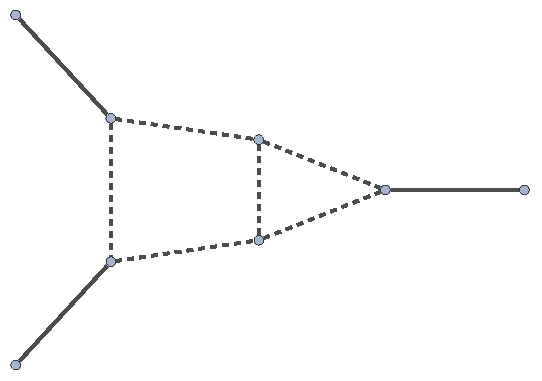
\includegraphics[width=0.6\linewidth]{img/0s3ekcbrughjs.pdf}
\end{figure}

\hypertarget{special-cases}{%
\subsubsection{Special cases}\label{special-cases}}

Not all loop integrals admit a graph representation. Furthermore, an
integral may have a weird momentum routing that cannot be automatically
recognized by the employed algorithm. Consider e.g.

\begin{Shaded}
\begin{Highlighting}[]
\NormalTok{topo }\ExtensionTok{=}\NormalTok{ FCTopology}\OperatorTok{[}\NormalTok{TRIX1}\OperatorTok{,} \OperatorTok{\{}\NormalTok{SFAD}\OperatorTok{[\{\{}\NormalTok{p2}\OperatorTok{,} \DecValTok{0}\OperatorTok{\},} \OperatorTok{\{}\DecValTok{0}\OperatorTok{,} \DecValTok{1}\OperatorTok{\},} \DecValTok{1}\OperatorTok{\}],}\NormalTok{ SFAD}\OperatorTok{[\{\{}\NormalTok{p1 }\SpecialCharTok{+}\NormalTok{ Q1}\OperatorTok{,} \DecValTok{0}\OperatorTok{\},} \OperatorTok{\{}\DecValTok{0}\OperatorTok{,} \DecValTok{1}\OperatorTok{\},} \DecValTok{1}\OperatorTok{\}],} 
\NormalTok{    SFAD}\OperatorTok{[\{\{}\NormalTok{p1 }\SpecialCharTok{+}\NormalTok{ p2 }\SpecialCharTok{+}\NormalTok{ Q1}\OperatorTok{,} \DecValTok{0}\OperatorTok{\},} \OperatorTok{\{}\DecValTok{0}\OperatorTok{,} \DecValTok{1}\OperatorTok{\},} \DecValTok{1}\OperatorTok{\}],}\NormalTok{ SFAD}\OperatorTok{[\{\{}\SpecialCharTok{{-}}\NormalTok{p1 }\SpecialCharTok{+}\NormalTok{ Q2}\OperatorTok{,} \DecValTok{0}\OperatorTok{\},} \OperatorTok{\{}\DecValTok{0}\OperatorTok{,} \DecValTok{1}\OperatorTok{\},} \DecValTok{1}\OperatorTok{\}],} 
\NormalTok{    SFAD}\OperatorTok{[\{\{}\SpecialCharTok{{-}}\NormalTok{p1 }\SpecialCharTok{{-}}\NormalTok{ p2 }\SpecialCharTok{+}\NormalTok{ Q2}\OperatorTok{,} \DecValTok{0}\OperatorTok{\},} \OperatorTok{\{}\DecValTok{0}\OperatorTok{,} \DecValTok{1}\OperatorTok{\},} \DecValTok{1}\OperatorTok{\}]\},} \OperatorTok{\{}\NormalTok{p1}\OperatorTok{,}\NormalTok{ p2}\OperatorTok{\},} \OperatorTok{\{}\NormalTok{Q1}\OperatorTok{,}\NormalTok{ Q2}\OperatorTok{\},} \OperatorTok{\{\},} \OperatorTok{\{\}]}
\end{Highlighting}
\end{Shaded}

\begin{dmath*}\breakingcomma
\text{FCTopology}\left(\text{TRIX1},\left\{\frac{1}{(\text{p2}^2+i \eta )},\frac{1}{((\text{p1}+\text{Q1})^2+i \eta )},\frac{1}{((\text{p1}+\text{p2}+\text{Q1})^2+i \eta )},\frac{1}{((\text{Q2}-\text{p1})^2+i \eta )},\frac{1}{((-\text{p1}-\text{p2}+\text{Q2})^2+i \eta )}\right\},\{\text{p1},\text{p2}\},\{\text{Q1},\text{Q2}\},\{\},\{\}\right)
\end{dmath*}

Here \texttt{FCLoopIntegralToGraph} has no way to know that the actual
momentum is Q1+Q2, i.e.~it is a 2- and not 3-point function

\begin{Shaded}
\begin{Highlighting}[]
\NormalTok{FCLoopIntegralToGraph}\OperatorTok{[}\NormalTok{topo}\OperatorTok{]}
\end{Highlighting}
\end{Shaded}

\begin{figure}[!ht]
\centering

\includegraphics[width=0.6\linewidth]{img/1f51tljs4rv5c.pdf}
\end{figure}

\begin{dmath*}\breakingcomma
\text{False}
\end{dmath*}

However, if we explicitly provide this information, in many cases the
function can still perform the proper reconstruction

\begin{Shaded}
\begin{Highlighting}[]
\NormalTok{FCLoopIntegralToGraph}\OperatorTok{[}\NormalTok{topo}\OperatorTok{,}\NormalTok{ Momentum }\OtherTok{{-}\textgreater{}} \OperatorTok{\{}\NormalTok{Q1 }\SpecialCharTok{+}\NormalTok{ Q2}\OperatorTok{\}]} 
 
\NormalTok{FCLoopGraphPlot}\OperatorTok{[}\SpecialCharTok{\%}\OperatorTok{]}
\end{Highlighting}
\end{Shaded}

\begin{dmath*}\breakingcomma
\left\{\{-3\to 2,-1\to 1,1\to 3,1\to 4,2\to 3,2\to 4,3\to 4\},\{\text{Q1}+\text{Q2},\text{Q1}+\text{Q2},\{\text{p1}+\text{Q1},1,0\},\{\text{Q2}-\text{p1},1,0\},\{\text{p1}+\text{p2}+\text{Q1},1,0\},\{-\text{p1}-\text{p2}+\text{Q2},1,0\},\{\text{p2},1,0\}\},\left\{0,0,\frac{1}{(\text{p2}^2+i \eta )},\frac{1}{((\text{p1}+\text{Q1})^2+i \eta )},\frac{1}{((\text{p1}+\text{p2}+\text{Q1})^2+i \eta )},\frac{1}{((\text{Q2}-\text{p1})^2+i \eta )},\frac{1}{((-\text{p1}-\text{p2}+\text{Q2})^2+i \eta )}\right\},1\right\}
\end{dmath*}

\begin{figure}[!ht]
\centering
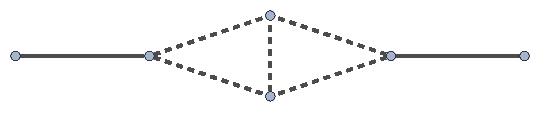
\includegraphics[width=0.6\linewidth]{img/1divxubmo2kg0.pdf}
\end{figure}

And here is another example. This NRQCD integral from
\href{https://arxiv.org/abs/1907.08227}{arXiv:1907.08227} looks like as
if it has only one external momentum flowing in

\begin{Shaded}
\begin{Highlighting}[]
\NormalTok{FCLoopIntegralToGraph}\OperatorTok{[}\NormalTok{FAD}\OperatorTok{[\{}\FunctionTok{k}\OperatorTok{,} \FunctionTok{m}\OperatorTok{\},} \FunctionTok{l} \SpecialCharTok{+} \FunctionTok{p}\OperatorTok{,} \FunctionTok{l} \SpecialCharTok{{-}} \FunctionTok{p}\OperatorTok{,} \FunctionTok{k} \SpecialCharTok{+} \FunctionTok{l}\OperatorTok{],} \OperatorTok{\{}\FunctionTok{k}\OperatorTok{,} \FunctionTok{l}\OperatorTok{\}]}
\end{Highlighting}
\end{Shaded}

\begin{figure}[!ht]
\centering

\includegraphics[width=0.6\linewidth]{img/0n5i5tvxn9tzb.pdf}
\end{figure}

\begin{dmath*}\breakingcomma
\text{False}
\end{dmath*}

while in reality there are two of them: \texttt{p} and \texttt{2p}

\begin{Shaded}
\begin{Highlighting}[]
\NormalTok{FCLoopIntegralToGraph}\OperatorTok{[}\NormalTok{FAD}\OperatorTok{[\{}\FunctionTok{k}\OperatorTok{,} \FunctionTok{m}\OperatorTok{\},} \FunctionTok{l} \SpecialCharTok{+} \FunctionTok{p}\OperatorTok{,} \FunctionTok{l} \SpecialCharTok{{-}} \FunctionTok{p}\OperatorTok{,} \FunctionTok{k} \SpecialCharTok{+} \FunctionTok{l}\OperatorTok{],} \OperatorTok{\{}\FunctionTok{k}\OperatorTok{,} \FunctionTok{l}\OperatorTok{\},} 
\NormalTok{   Momentum }\OtherTok{{-}\textgreater{}} \OperatorTok{\{}\DecValTok{2} \FunctionTok{p}\OperatorTok{,} \FunctionTok{p}\OperatorTok{\},}\NormalTok{ FCE }\OtherTok{{-}\textgreater{}} \ConstantTok{True}\OperatorTok{]} 
 
\NormalTok{FCLoopGraphPlot}\OperatorTok{[}\SpecialCharTok{\%}\OperatorTok{]}
\end{Highlighting}
\end{Shaded}

\begin{dmath*}\breakingcomma
\left\{\{-4\to 3,-2\to 2,-1\to 1,1\to 2,1\to 3,2\to 3,2\to 3\},\left\{3 p,2 p,p,\{l+p,1,0\},\{l-p,1,0\},\{k+l,1,0\},\left\{k,1,-m^2\right\}\right\},\left\{0,0,0,\frac{1}{((l+p)^2+i \eta )},\frac{1}{((k+l)^2+i \eta )},\frac{1}{((l-p)^2+i \eta )},\frac{1}{(k^2-m^2+i \eta )}\right\},1\right\}
\end{dmath*}

\begin{figure}[!ht]
\centering
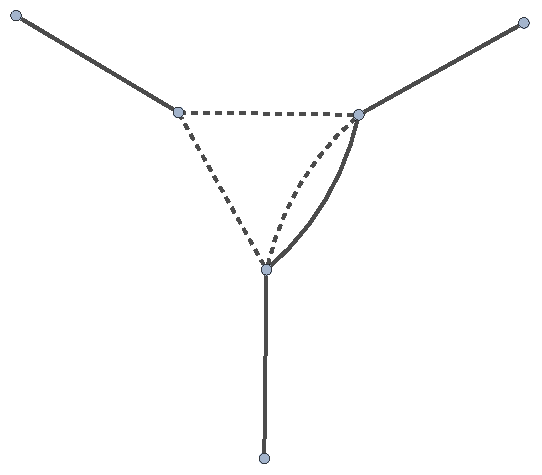
\includegraphics[width=0.6\linewidth]{img/00vlxernf5uq8.pdf}
\end{figure}

In this case the correct form of the external momentum can be deduced
upon performing some elementary shifts. The direct application of the
function fails

\begin{Shaded}
\begin{Highlighting}[]
\NormalTok{ex }\ExtensionTok{=}\NormalTok{ FCTopology}\OperatorTok{[}\NormalTok{topo1X12679}\OperatorTok{,} \OperatorTok{\{}\NormalTok{SFAD}\OperatorTok{[\{\{}\NormalTok{p1}\OperatorTok{,} \DecValTok{0}\OperatorTok{\},} \OperatorTok{\{}\DecValTok{0}\OperatorTok{,} \DecValTok{1}\OperatorTok{\},} \DecValTok{1}\OperatorTok{\}],}\NormalTok{ SFAD}\OperatorTok{[\{\{}\NormalTok{p2 }\SpecialCharTok{+}\NormalTok{ p3}\OperatorTok{,} \DecValTok{0}\OperatorTok{\},} \OperatorTok{\{}\DecValTok{0}\OperatorTok{,} \DecValTok{1}\OperatorTok{\},} \DecValTok{1}\OperatorTok{\}],} 
\NormalTok{    SFAD}\OperatorTok{[\{\{}\NormalTok{p2 }\SpecialCharTok{{-}} \FunctionTok{Q}\OperatorTok{,} \DecValTok{0}\OperatorTok{\},} \OperatorTok{\{}\DecValTok{0}\OperatorTok{,} \DecValTok{1}\OperatorTok{\},} \DecValTok{1}\OperatorTok{\}],}\NormalTok{ SFAD}\OperatorTok{[\{\{}\NormalTok{p1 }\SpecialCharTok{+}\NormalTok{ p3 }\SpecialCharTok{{-}} \FunctionTok{Q}\OperatorTok{,} \DecValTok{0}\OperatorTok{\},} \OperatorTok{\{}\DecValTok{0}\OperatorTok{,} \DecValTok{1}\OperatorTok{\},} \DecValTok{1}\OperatorTok{\}]\},} \OperatorTok{\{}\NormalTok{p1}\OperatorTok{,}\NormalTok{ p2}\OperatorTok{,}\NormalTok{ p3}\OperatorTok{\},} \OperatorTok{\{}\FunctionTok{Q}\OperatorTok{\},} \OperatorTok{\{\},} \OperatorTok{\{\}]}
\end{Highlighting}
\end{Shaded}

\begin{dmath*}\breakingcomma
\text{FCTopology}\left(\text{topo1X12679},\left\{\frac{1}{(\text{p1}^2+i \eta )},\frac{1}{((\text{p2}+\text{p3})^2+i \eta )},\frac{1}{((\text{p2}-Q)^2+i \eta )},\frac{1}{((\text{p1}+\text{p3}-Q)^2+i \eta )}\right\},\{\text{p1},\text{p2},\text{p3}\},\{Q\},\{\},\{\}\right)
\end{dmath*}

\begin{Shaded}
\begin{Highlighting}[]
\NormalTok{FCLoopIntegralToGraph}\OperatorTok{[}\NormalTok{ex}\OperatorTok{]}
\end{Highlighting}
\end{Shaded}

\begin{figure}[!ht]
\centering

\includegraphics[width=0.6\linewidth]{img/112s7t3w9k2l3.pdf}
\end{figure}

\begin{dmath*}\breakingcomma
\text{False}
\end{dmath*}

Yet let us consider

\begin{Shaded}
\begin{Highlighting}[]
\NormalTok{exShifted }\ExtensionTok{=}\NormalTok{ FCReplaceMomenta}\OperatorTok{[}\NormalTok{ex}\OperatorTok{,} \OperatorTok{\{}\NormalTok{p2 }\OtherTok{{-}\textgreater{}}\NormalTok{ p2 }\SpecialCharTok{{-}}\NormalTok{ p3 }\SpecialCharTok{+}\NormalTok{ p1 }\SpecialCharTok{{-}} \FunctionTok{Q}\OperatorTok{,}\NormalTok{ p3 }\OtherTok{{-}\textgreater{}}\NormalTok{ p3 }\SpecialCharTok{{-}}\NormalTok{ p1 }\SpecialCharTok{+} \FunctionTok{Q}\OperatorTok{\}]}
\end{Highlighting}
\end{Shaded}

\begin{dmath*}\breakingcomma
\text{FCTopology}\left(\text{topo1X12679},\left\{\frac{1}{(\text{p1}^2+i \eta )},\frac{1}{(\text{p2}^2+i \eta )},\frac{1}{((\text{p1}+\text{p2}-\text{p3}-2 Q)^2+i \eta )},\frac{1}{(\text{p3}^2+i \eta )}\right\},\{\text{p1},\text{p2},\text{p3}\},\{Q\},\{\},\{\}\right)
\end{dmath*}

Now we immediately see that the proper external momentum to consider is
\texttt{2Q} instead of just \texttt{Q}

\begin{Shaded}
\begin{Highlighting}[]
\NormalTok{FCLoopIntegralToGraph}\OperatorTok{[}\NormalTok{exShifted}\OperatorTok{,}\NormalTok{ Momentum }\OtherTok{{-}\textgreater{}} \OperatorTok{\{}\DecValTok{2} \FunctionTok{Q}\OperatorTok{\}]} 
 
\NormalTok{FCLoopGraphPlot}\OperatorTok{[}\SpecialCharTok{\%}\OperatorTok{]}
\end{Highlighting}
\end{Shaded}

\begin{dmath*}\breakingcomma
\left\{\{-3\to 2,-1\to 1,1\to 2,1\to 2,1\to 2,1\to 2\},\{2 Q,2 Q,\{\text{p3},1,0\},\{\text{p2},1,0\},\{\text{p1},1,0\},\{\text{p1}+\text{p2}-\text{p3}-2 Q,1,0\}\},\left\{0,0,\frac{1}{(\text{p3}^2+i \eta )},\frac{1}{(\text{p2}^2+i \eta )},\frac{1}{(\text{p1}^2+i \eta )},\frac{1}{((\text{p1}+\text{p2}-\text{p3}-2 Q)^2+i \eta )}\right\},1\right\}
\end{dmath*}

\begin{figure}[!ht]
\centering
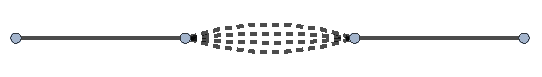
\includegraphics[width=0.6\linewidth]{img/0epvj32a3mspb.pdf}
\end{figure}

When dealing with products of tadpole integrals, the function may not
always recognize that the appearing external momenta are spurious. For
example, here there is no \texttt{q} momentum flowing through any of the
lines

\begin{Shaded}
\begin{Highlighting}[]
\NormalTok{int }\ExtensionTok{=}\NormalTok{ SFAD}\OperatorTok{[\{\{}\NormalTok{ p1}\OperatorTok{,} \DecValTok{0}\OperatorTok{\},} \OperatorTok{\{}\NormalTok{mg}\SpecialCharTok{\^{}}\DecValTok{2}\OperatorTok{,} \DecValTok{1}\OperatorTok{\},} \DecValTok{1}\OperatorTok{\}]}\NormalTok{ SFAD}\OperatorTok{[\{\{}\NormalTok{ p3}\OperatorTok{,} \SpecialCharTok{{-}}\DecValTok{2}\NormalTok{ p3 . }\FunctionTok{q}\OperatorTok{\},} \OperatorTok{\{}\DecValTok{0}\OperatorTok{,} \DecValTok{1}\OperatorTok{\},} \DecValTok{1}\OperatorTok{\}]} 
 
\NormalTok{FCLoopIntegralToGraph}\OperatorTok{[}\NormalTok{int}\OperatorTok{,} \OperatorTok{\{}\NormalTok{p1}\OperatorTok{,}\NormalTok{ p3}\OperatorTok{\}]}
\end{Highlighting}
\end{Shaded}

\begin{dmath*}\breakingcomma
\frac{1}{(\text{p1}^2-\text{mg}^2+i \eta ) (\text{p3}^2-2 (\text{p3}\cdot q)+i \eta )}
\end{dmath*}

\begin{figure}[!ht]
\centering

\includegraphics[width=0.6\linewidth]{img/04u9cv0rn5xej.pdf}
\end{figure}

\begin{dmath*}\breakingcomma
\text{False}
\end{dmath*}

In this case we may explicitly tell the function that this integral
doesn't depend on any external momenta

\begin{Shaded}
\begin{Highlighting}[]
\NormalTok{FCLoopIntegralToGraph}\OperatorTok{[}\NormalTok{int}\OperatorTok{,} \OperatorTok{\{}\NormalTok{p1}\OperatorTok{,}\NormalTok{ p3}\OperatorTok{\},}\NormalTok{ Momentum }\OtherTok{{-}\textgreater{}} \OperatorTok{\{\}]} 
 
\NormalTok{FCLoopGraphPlot}\OperatorTok{[}\SpecialCharTok{\%}\OperatorTok{]}
\end{Highlighting}
\end{Shaded}

\begin{dmath*}\breakingcomma
\left\{\{1\to 1,1\to 1\},\left(
\begin{array}{ccc}
 \;\text{p1} & 1 & -\text{mg}^2 \\
 \;\text{p3}-q & 1 & 0 \\
\end{array}
\right),\left\{\frac{1}{(\text{p1}^2-\text{mg}^2+i \eta )},\frac{1}{(\text{p3}^2-2 (\text{p3}\cdot q)+i \eta )}\right\},1\right\}
\end{dmath*}

\begin{figure}[!ht]
\centering
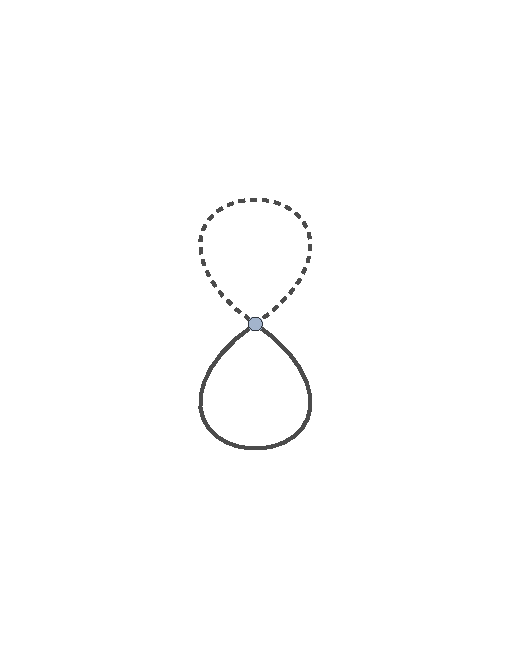
\includegraphics[width=0.6\linewidth]{img/0x74zmssj7d9o.pdf}
\end{figure}

\hypertarget{eye-candy}{%
\subsubsection{Eye candy}\label{eye-candy}}

The \texttt{Style} option can be used to label lines carrying different
masses in a particular way

\begin{Shaded}
\begin{Highlighting}[]
\FunctionTok{OptionValue}\OperatorTok{[}\NormalTok{FCLoopGraphPlot}\OperatorTok{,} \FunctionTok{Style}\OperatorTok{]}
\end{Highlighting}
\end{Shaded}

\begin{dmath*}\breakingcomma
\{\{\text{InternalLine},\_,\_,0\}:\to \{\text{Dashed},\text{Thick},\text{Black}\},\{\text{InternalLine},\_,\_,\text{FeynCalc$\grave{ }$FCLoopGraphPlot$\grave{ }$Private$\grave{ }$mm$\_$}\;\text{/;}\;\text{FeynCalc$\grave{ }$FCLoopGraphPlot$\grave{ }$Private$\grave{ }$mm}\;\text{=!=}0\}:\to \{\text{Thick},\text{Black}\},\{\text{ExternalLine},\_\}:\to \{\text{Thick},\text{Black}\}\}
\end{dmath*}

When dealing with factorizing integral it might be necessary to increase
\texttt{VertexDegree} to \texttt{7} or \texttt{8} (or even a higher
value, depending on the integrals)

\begin{Shaded}
\begin{Highlighting}[]
\NormalTok{FCLoopIntegralToGraph}\OperatorTok{[}\NormalTok{FAD}\OperatorTok{[\{}\NormalTok{p1}\OperatorTok{,}\NormalTok{ m1}\OperatorTok{\}]}\NormalTok{ FAD}\OperatorTok{[\{}\NormalTok{p2}\OperatorTok{,}\NormalTok{ m2}\OperatorTok{\}],} \OperatorTok{\{}\NormalTok{p1}\OperatorTok{,}\NormalTok{ p2}\OperatorTok{\}]}
\NormalTok{FCLoopGraphPlot}\OperatorTok{[}\SpecialCharTok{\%}\OperatorTok{]}
\end{Highlighting}
\end{Shaded}

\begin{dmath*}\breakingcomma
\left\{\{1\to 1,1\to 1\},\left(
\begin{array}{ccc}
 \;\text{p2} & 1 & -\text{m2}^2 \\
 \;\text{p1} & 1 & -\text{m1}^2 \\
\end{array}
\right),\left\{\frac{1}{(\text{p2}^2-\text{m2}^2+i \eta )},\frac{1}{(\text{p1}^2-\text{m1}^2+i \eta )}\right\},1\right\}
\end{dmath*}

\begin{figure}[!ht]
\centering
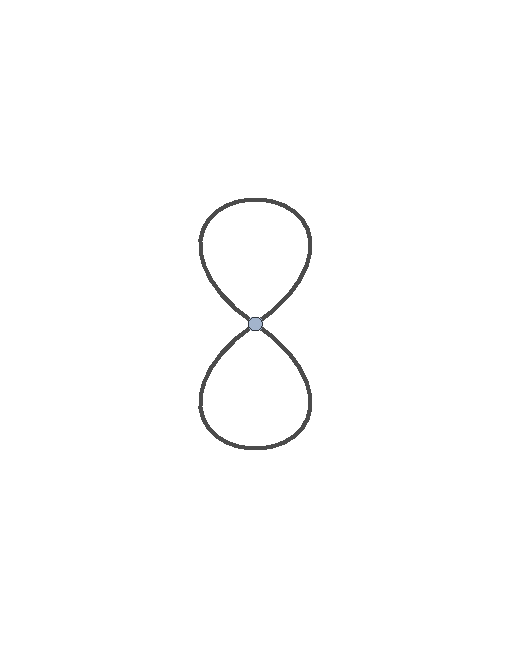
\includegraphics[width=0.6\linewidth]{img/0mz3vndnoqr9r.pdf}
\end{figure}

\begin{Shaded}
\begin{Highlighting}[]
\NormalTok{FCLoopIntegralToGraph}\OperatorTok{[}\NormalTok{FAD}\OperatorTok{[\{}\NormalTok{p1}\OperatorTok{,}\NormalTok{ m1}\OperatorTok{\}]}\NormalTok{ FAD}\OperatorTok{[\{}\NormalTok{p2}\OperatorTok{,}\NormalTok{ m2}\OperatorTok{\}]}\NormalTok{ FAD}\OperatorTok{[}\NormalTok{p3}\OperatorTok{,}\NormalTok{ p3 }\SpecialCharTok{+} \FunctionTok{q}\OperatorTok{],} \OperatorTok{\{}\NormalTok{p1}\OperatorTok{,}\NormalTok{ p2}\OperatorTok{,}\NormalTok{ p3}\OperatorTok{\},} 
   \FunctionTok{VertexDegree} \OtherTok{{-}\textgreater{}} \DecValTok{7}\OperatorTok{]} 
 
\NormalTok{FCLoopGraphPlot}\OperatorTok{[}\SpecialCharTok{\%}\OperatorTok{]}
\end{Highlighting}
\end{Shaded}

\begin{dmath*}\breakingcomma
\left\{\{-3\to 2,-1\to 1,1\to 2,1\to 2,2\to 2,2\to 2\},\left\{q,q,\{\text{p3},1,0\},\{\text{p3}+q,1,0\},\left\{\text{p2},1,-\text{m2}^2\right\},\left\{\text{p1},1,-\text{m1}^2\right\}\right\},\left\{0,0,\frac{1}{(\text{p3}^2+i \eta )},\frac{1}{((\text{p3}+q)^2+i \eta )},\frac{1}{(\text{p2}^2-\text{m2}^2+i \eta )},\frac{1}{(\text{p1}^2-\text{m1}^2+i \eta )}\right\},1\right\}
\end{dmath*}

\begin{figure}[!ht]
\centering
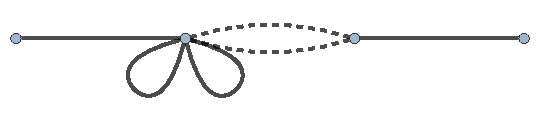
\includegraphics[width=0.6\linewidth]{img/17a2ldq41hi7m.pdf}
\end{figure}

\begin{Shaded}
\begin{Highlighting}[]
\NormalTok{FCLoopIntegralToGraph}\OperatorTok{[}\NormalTok{FAD}\OperatorTok{[\{}\NormalTok{p1}\OperatorTok{,}\NormalTok{ m1}\OperatorTok{\}]}\NormalTok{ FAD}\OperatorTok{[\{}\NormalTok{p2}\OperatorTok{,}\NormalTok{ m2}\OperatorTok{\}]}\NormalTok{ FAD}\OperatorTok{[}\NormalTok{p3}\OperatorTok{,}\NormalTok{ p3 }\SpecialCharTok{+} \FunctionTok{q}\OperatorTok{]}\NormalTok{ FAD}\OperatorTok{[\{}\NormalTok{p4}\OperatorTok{,}\NormalTok{ m4}\OperatorTok{\}],} 
   \OperatorTok{\{}\NormalTok{p1}\OperatorTok{,}\NormalTok{ p2}\OperatorTok{,}\NormalTok{ p3}\OperatorTok{,}\NormalTok{ p4}\OperatorTok{\},} \FunctionTok{VertexDegree} \OtherTok{{-}\textgreater{}} \DecValTok{9}\OperatorTok{]} 
 
\NormalTok{FCLoopGraphPlot}\OperatorTok{[}\SpecialCharTok{\%}\OperatorTok{]}
\end{Highlighting}
\end{Shaded}

\begin{dmath*}\breakingcomma
\left\{\{-3\to 2,-1\to 1,1\to 2,1\to 2,2\to 2,2\to 2,2\to 2\},\left\{q,q,\{\text{p3},1,0\},\{\text{p3}+q,1,0\},\left\{\text{p4},1,-\text{m4}^2\right\},\left\{\text{p2},1,-\text{m2}^2\right\},\left\{\text{p1},1,-\text{m1}^2\right\}\right\},\left\{0,0,\frac{1}{(\text{p3}^2+i \eta )},\frac{1}{((\text{p3}+q)^2+i \eta )},\frac{1}{(\text{p4}^2-\text{m4}^2+i \eta )},\frac{1}{(\text{p2}^2-\text{m2}^2+i \eta )},\frac{1}{(\text{p1}^2-\text{m1}^2+i \eta )}\right\},1\right\}
\end{dmath*}

\begin{figure}[!ht]
\centering
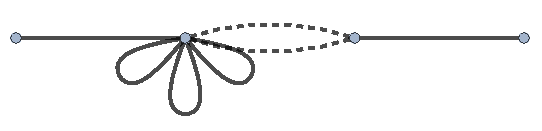
\includegraphics[width=0.6\linewidth]{img/09zo33bciw4fw.pdf}
\end{figure}

Here we choose to use thick dashed blue and red lines for massive lines
containing \texttt{mc} and \texttt{mg} respectively. The massless lines
are black an dashed.

\begin{Shaded}
\begin{Highlighting}[]
\NormalTok{FCLoopIntegralToGraph}\OperatorTok{[}\NormalTok{ FAD}\OperatorTok{[\{}\NormalTok{k2}\OperatorTok{,}\NormalTok{ mb}\OperatorTok{\},} \OperatorTok{\{}\NormalTok{k3}\OperatorTok{\},} \OperatorTok{\{}\NormalTok{k1 }\SpecialCharTok{{-}} \FunctionTok{q}\OperatorTok{,}\NormalTok{ mc}\OperatorTok{\},} \OperatorTok{\{}\NormalTok{k1 }\SpecialCharTok{{-}}\NormalTok{ k2}\OperatorTok{,}\NormalTok{ mc}\OperatorTok{\},} \OperatorTok{\{}\NormalTok{k2 }\SpecialCharTok{{-}}\NormalTok{ k3}\OperatorTok{\}],} \OperatorTok{\{}\NormalTok{k1}\OperatorTok{,}\NormalTok{ k2}\OperatorTok{,}\NormalTok{ k3}\OperatorTok{\}]} 
 
\FunctionTok{Magnify}\OperatorTok{[}\NormalTok{FCLoopGraphPlot}\OperatorTok{[}\SpecialCharTok{\%}\OperatorTok{,} \FunctionTok{GraphPlot} \OtherTok{{-}\textgreater{}} \OperatorTok{\{}\FunctionTok{MultiedgeStyle} \OtherTok{{-}\textgreater{}} \FloatTok{0.35}\OperatorTok{,} \FunctionTok{Frame} \OtherTok{{-}\textgreater{}} \ConstantTok{True}\OperatorTok{\},} 
   \FunctionTok{Style} \OtherTok{{-}\textgreater{}} \OperatorTok{\{\{}\StringTok{"InternalLine"}\OperatorTok{,}\NormalTok{ \_}\OperatorTok{,}\NormalTok{ \_}\OperatorTok{,} \AttributeTok{mm\_} \SpecialCharTok{/}\NormalTok{; ! }\FunctionTok{FreeQ}\OperatorTok{[}\NormalTok{mm}\OperatorTok{,}\NormalTok{ mg}\OperatorTok{]\}} \OtherTok{{-}\textgreater{}} \OperatorTok{\{}\FunctionTok{Red}\OperatorTok{,} \FunctionTok{Thick}\OperatorTok{,} \FunctionTok{Dashed}\OperatorTok{\},} 
     \OperatorTok{\{}\StringTok{"InternalLine"}\OperatorTok{,}\NormalTok{ \_}\OperatorTok{,}\NormalTok{ \_}\OperatorTok{,} \AttributeTok{mm\_} \SpecialCharTok{/}\NormalTok{; ! }\FunctionTok{FreeQ}\OperatorTok{[}\NormalTok{mm}\OperatorTok{,}\NormalTok{ mc}\OperatorTok{]\}} \OtherTok{{-}\textgreater{}} \OperatorTok{\{}\FunctionTok{Blue}\OperatorTok{,} \FunctionTok{Thick}\OperatorTok{,} \FunctionTok{Dashed}\OperatorTok{\}\}],} \FloatTok{1.5}\OperatorTok{]}
\end{Highlighting}
\end{Shaded}

\begin{dmath*}\breakingcomma
\left\{\{-3\to 2,-1\to 1,1\to 2,1\to 2,1\to 3,2\to 3,2\to 3\},\left\{q,q,\left\{\text{k1}-q,1,-\text{mc}^2\right\},\left\{\text{k1}-\text{k2},1,-\text{mc}^2\right\},\left\{\text{k2},1,-\text{mb}^2\right\},\{\text{k3},1,0\},\{\text{k2}-\text{k3},1,0\}\right\},\left\{0,0,\frac{1}{(\text{k3}^2+i \eta )},\frac{1}{((\text{k2}-\text{k3})^2+i \eta )},\frac{1}{(\text{k2}^2-\text{mb}^2+i \eta )},\frac{1}{((\text{k1}-q)^2-\text{mc}^2+i \eta )},\frac{1}{((\text{k1}-\text{k2})^2-\text{mc}^2+i \eta )}\right\},1\right\}
\end{dmath*}

\begin{figure}[!ht]
\centering
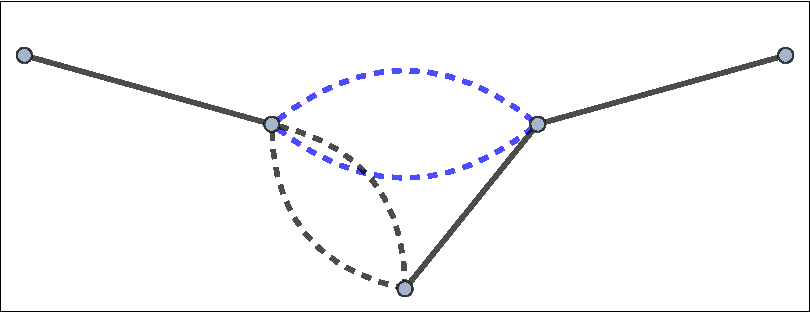
\includegraphics[width=0.6\linewidth]{img/0dmivk9ohasqm.pdf}
\end{figure}

\begin{Shaded}
\begin{Highlighting}[]
\NormalTok{FCLoopIntegralToGraph}\OperatorTok{[}\NormalTok{ FAD}\OperatorTok{[\{}\NormalTok{k2}\OperatorTok{,}\NormalTok{ mg}\OperatorTok{\},} \OperatorTok{\{}\NormalTok{k3}\OperatorTok{,}\NormalTok{ mc}\OperatorTok{\},} \OperatorTok{\{}\NormalTok{k1}\OperatorTok{,} \FunctionTok{q}\OperatorTok{\},} \OperatorTok{\{}\NormalTok{k1 }\SpecialCharTok{{-}}\NormalTok{ k2}\OperatorTok{\},} \OperatorTok{\{}\NormalTok{k2 }\SpecialCharTok{{-}}\NormalTok{ k3}\OperatorTok{,}\NormalTok{ mc}\OperatorTok{\}],} \OperatorTok{\{}\NormalTok{k1}\OperatorTok{,}\NormalTok{ k2}\OperatorTok{,}\NormalTok{k3}\OperatorTok{\}]} 
 
\FunctionTok{Magnify}\OperatorTok{[}\NormalTok{FCLoopGraphPlot}\OperatorTok{[}\SpecialCharTok{\%}\OperatorTok{,} \FunctionTok{GraphPlot} \OtherTok{{-}\textgreater{}} \OperatorTok{\{}\FunctionTok{MultiedgeStyle} \OtherTok{{-}\textgreater{}} \FloatTok{0.35}\OperatorTok{,} \FunctionTok{Frame} \OtherTok{{-}\textgreater{}} \ConstantTok{True}\OperatorTok{\},} 
   \FunctionTok{Style} \OtherTok{{-}\textgreater{}} \OperatorTok{\{\{}\StringTok{"InternalLine"}\OperatorTok{,}\NormalTok{ \_}\OperatorTok{,}\NormalTok{ \_}\OperatorTok{,} \AttributeTok{mm\_} \SpecialCharTok{/}\NormalTok{; ! }\FunctionTok{FreeQ}\OperatorTok{[}\NormalTok{mm}\OperatorTok{,}\NormalTok{ mg}\OperatorTok{]\}} \OtherTok{{-}\textgreater{}} \OperatorTok{\{}\FunctionTok{Red}\OperatorTok{,} \FunctionTok{Thick}\OperatorTok{,} \FunctionTok{Dashed}\OperatorTok{\},} 
     \OperatorTok{\{}\StringTok{"InternalLine"}\OperatorTok{,}\NormalTok{ \_}\OperatorTok{,}\NormalTok{ \_}\OperatorTok{,} \AttributeTok{mm\_} \SpecialCharTok{/}\NormalTok{; ! }\FunctionTok{FreeQ}\OperatorTok{[}\NormalTok{mm}\OperatorTok{,}\NormalTok{ mc}\OperatorTok{]\}} \OtherTok{{-}\textgreater{}} \OperatorTok{\{}\FunctionTok{Blue}\OperatorTok{,} \FunctionTok{Thick}\OperatorTok{,} \FunctionTok{Dashed}\OperatorTok{\}\}],} \FloatTok{1.5}\OperatorTok{]}
\end{Highlighting}
\end{Shaded}

\begin{dmath*}\breakingcomma
\left\{\{1\to 2,1\to 3,1\to 3,2\to 3,2\to 3\},\left(
\begin{array}{ccc}
 \;\text{k2} & 1 & -\text{mg}^2 \\
 \;\text{k3} & 1 & -\text{mc}^2 \\
 \;\text{k2}-\text{k3} & 1 & -\text{mc}^2 \\
 \;\text{k1}-\text{k2} & 1 & 0 \\
 \;\text{k1} & 1 & -q^2 \\
\end{array}
\right),\left\{\frac{1}{(\text{k3}^2-\text{mc}^2+i \eta )},\frac{1}{(\text{k2}^2-\text{mg}^2+i \eta )},\frac{1}{((\text{k1}-\text{k2})^2+i \eta )},\frac{1}{(\text{k1}^2-q^2+i \eta )},\frac{1}{((\text{k2}-\text{k3})^2-\text{mc}^2+i \eta )}\right\},1\right\}
\end{dmath*}

\begin{figure}[!ht]
\centering
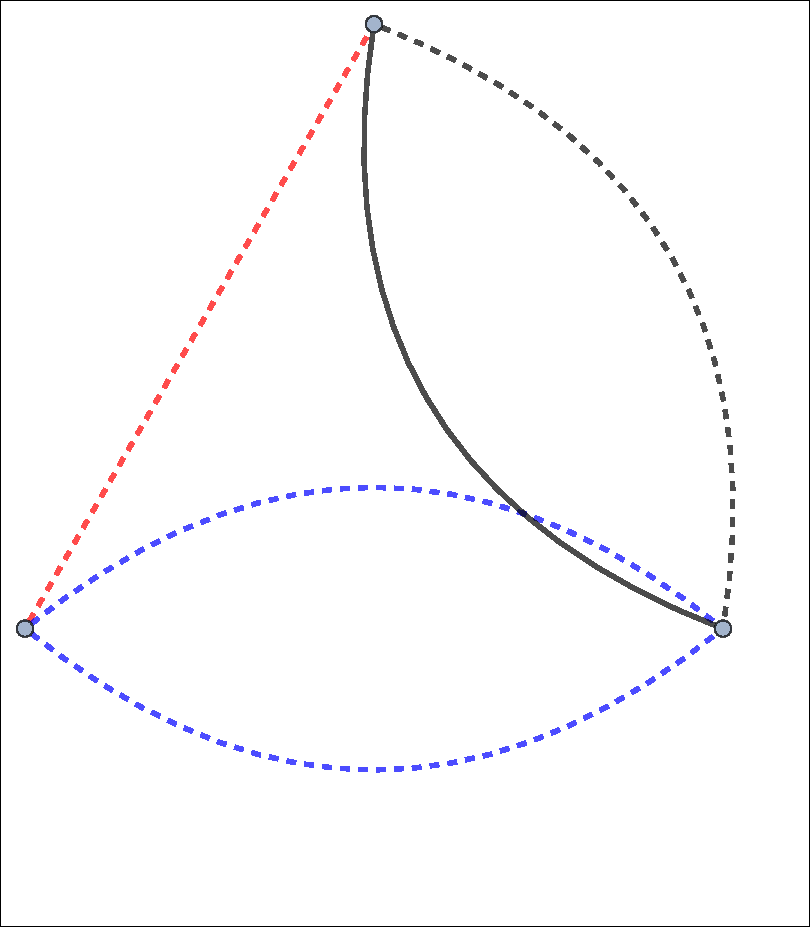
\includegraphics[width=0.6\linewidth]{img/1ntnpbkdk69j9.pdf}
\end{figure}

\begin{Shaded}
\begin{Highlighting}[]
\NormalTok{FCLoopIntegralToGraph}\OperatorTok{[}\NormalTok{ FAD}\OperatorTok{[\{}\NormalTok{k2}\OperatorTok{,}\NormalTok{ mg}\OperatorTok{\},} \OperatorTok{\{}\NormalTok{k3}\OperatorTok{,}\NormalTok{ mc}\OperatorTok{\},} \OperatorTok{\{}\NormalTok{k1 }\SpecialCharTok{{-}} \FunctionTok{q}\OperatorTok{\},} \OperatorTok{\{}\NormalTok{k2 }\SpecialCharTok{{-}} \FunctionTok{q}\OperatorTok{,}\NormalTok{ mb}\OperatorTok{\},} \OperatorTok{\{}\NormalTok{k1 }\SpecialCharTok{{-}}\NormalTok{ k2}\OperatorTok{\},} \OperatorTok{\{}\NormalTok{k2 }\SpecialCharTok{{-}}\NormalTok{ k3}\OperatorTok{,}\NormalTok{mc}\OperatorTok{\}],} 
   \OperatorTok{\{}\NormalTok{k1}\OperatorTok{,}\NormalTok{ k2}\OperatorTok{,}\NormalTok{ k3}\OperatorTok{\}]} 
 
\FunctionTok{Magnify}\OperatorTok{[}\NormalTok{FCLoopGraphPlot}\OperatorTok{[}\SpecialCharTok{\%}\OperatorTok{,} \FunctionTok{GraphPlot} \OtherTok{{-}\textgreater{}} \OperatorTok{\{}\FunctionTok{MultiedgeStyle} \OtherTok{{-}\textgreater{}} \FloatTok{0.35}\OperatorTok{,} \FunctionTok{Frame} \OtherTok{{-}\textgreater{}} \ConstantTok{True}\OperatorTok{\},} 
   \FunctionTok{Style} \OtherTok{{-}\textgreater{}} \OperatorTok{\{\{}\StringTok{"InternalLine"}\OperatorTok{,}\NormalTok{ \_}\OperatorTok{,}\NormalTok{ \_}\OperatorTok{,} \AttributeTok{mm\_} \SpecialCharTok{/}\NormalTok{; ! }\FunctionTok{FreeQ}\OperatorTok{[}\NormalTok{mm}\OperatorTok{,}\NormalTok{ mg}\OperatorTok{]\}} \OtherTok{{-}\textgreater{}} \OperatorTok{\{}\FunctionTok{Red}\OperatorTok{,} \FunctionTok{Thick}\OperatorTok{,} \FunctionTok{Dashed}\OperatorTok{\},} 
     \OperatorTok{\{}\StringTok{"InternalLine"}\OperatorTok{,}\NormalTok{ \_}\OperatorTok{,}\NormalTok{ \_}\OperatorTok{,} \AttributeTok{mm\_} \SpecialCharTok{/}\NormalTok{; ! }\FunctionTok{FreeQ}\OperatorTok{[}\NormalTok{mm}\OperatorTok{,}\NormalTok{ mc}\OperatorTok{]\}} \OtherTok{{-}\textgreater{}} \OperatorTok{\{}\FunctionTok{Blue}\OperatorTok{,} \FunctionTok{Thick}\OperatorTok{,} \FunctionTok{Dashed}\OperatorTok{\}\}],} \FloatTok{1.5}\OperatorTok{]}
\end{Highlighting}
\end{Shaded}

\begin{dmath*}\breakingcomma
\left\{\{-3\to 2,-1\to 1,1\to 3,1\to 4,2\to 3,2\to 3,2\to 4,2\to 4\},\left\{q,q,\left\{\text{k2}-q,1,-\text{mb}^2\right\},\left\{\text{k2},1,-\text{mg}^2\right\},\{\text{k1}-q,1,0\},\{\text{k1}-\text{k2},1,0\},\left\{\text{k3},1,-\text{mc}^2\right\},\left\{\text{k2}-\text{k3},1,-\text{mc}^2\right\}\right\},\left\{0,0,\frac{1}{((\text{k1}-q)^2+i \eta )},\frac{1}{(\text{k3}^2-\text{mc}^2+i \eta )},\frac{1}{(\text{k2}^2-\text{mg}^2+i \eta )},\frac{1}{((\text{k1}-\text{k2})^2+i \eta )},\frac{1}{((\text{k2}-q)^2-\text{mb}^2+i \eta )},\frac{1}{((\text{k2}-\text{k3})^2-\text{mc}^2+i \eta )}\right\},1\right\}
\end{dmath*}

\begin{figure}[!ht]
\centering
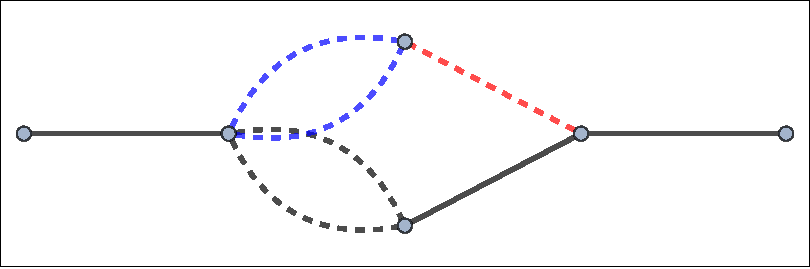
\includegraphics[width=0.6\linewidth]{img/0isqi3dlxey8z.pdf}
\end{figure}

\begin{Shaded}
\begin{Highlighting}[]
\NormalTok{FCLoopIntegralToGraph}\OperatorTok{[}\NormalTok{ FAD}\OperatorTok{[\{}\NormalTok{k2}\OperatorTok{,} \DecValTok{0}\OperatorTok{,} \DecValTok{2}\OperatorTok{\},} \OperatorTok{\{}\NormalTok{k1 }\SpecialCharTok{{-}} \FunctionTok{q}\OperatorTok{\},} \OperatorTok{\{}\NormalTok{k1 }\SpecialCharTok{{-}}\NormalTok{ k3}\OperatorTok{,}\NormalTok{ mc}\OperatorTok{\},} \OperatorTok{\{}\NormalTok{k2 }\SpecialCharTok{{-}}\NormalTok{ k3}\OperatorTok{,}\NormalTok{ mc}\OperatorTok{\}],} \OperatorTok{\{}\NormalTok{k1}\OperatorTok{,}\NormalTok{ k2}\OperatorTok{,}\NormalTok{ k3}\OperatorTok{\}]} 
 
\FunctionTok{Magnify}\OperatorTok{[}\NormalTok{FCLoopGraphPlot}\OperatorTok{[}\SpecialCharTok{\%}\OperatorTok{,} \FunctionTok{GraphPlot} \OtherTok{{-}\textgreater{}} \OperatorTok{\{}\FunctionTok{MultiedgeStyle} \OtherTok{{-}\textgreater{}} \FloatTok{0.35}\OperatorTok{,} \FunctionTok{Frame} \OtherTok{{-}\textgreater{}} \ConstantTok{True}\OperatorTok{\},} 
   \FunctionTok{Style} \OtherTok{{-}\textgreater{}} \OperatorTok{\{\{}\StringTok{"InternalLine"}\OperatorTok{,}\NormalTok{ \_}\OperatorTok{,}\NormalTok{ \_}\OperatorTok{,} \AttributeTok{mm\_} \SpecialCharTok{/}\NormalTok{; ! }\FunctionTok{FreeQ}\OperatorTok{[}\NormalTok{mm}\OperatorTok{,}\NormalTok{ mg}\OperatorTok{]\}} \OtherTok{{-}\textgreater{}} \OperatorTok{\{}\FunctionTok{Red}\OperatorTok{,} \FunctionTok{Thick}\OperatorTok{,} \FunctionTok{Dashed}\OperatorTok{\},} 
     \OperatorTok{\{}\StringTok{"InternalLine"}\OperatorTok{,}\NormalTok{ \_}\OperatorTok{,}\NormalTok{ \_}\OperatorTok{,} \AttributeTok{mm\_} \SpecialCharTok{/}\NormalTok{; ! }\FunctionTok{FreeQ}\OperatorTok{[}\NormalTok{mm}\OperatorTok{,}\NormalTok{ mc}\OperatorTok{]\}} \OtherTok{{-}\textgreater{}} \OperatorTok{\{}\FunctionTok{Blue}\OperatorTok{,} \FunctionTok{Thick}\OperatorTok{,} \FunctionTok{Dashed}\OperatorTok{\}\}],} \FloatTok{1.5}\OperatorTok{]}
\end{Highlighting}
\end{Shaded}

\begin{dmath*}\breakingcomma
\left\{\{-3\to 2,-1\to 1,1\to 2,1\to 2,1\to 2,1\to 2\},\left\{q,q,\{\text{k2},2,0\},\{\text{k1}-q,1,0\},\left\{\text{k2}-\text{k3},1,-\text{mc}^2\right\},\left\{\text{k1}-\text{k3},1,-\text{mc}^2\right\}\right\},\left\{0,0,\frac{1}{(\text{k2}^2+i \eta )},\frac{1}{((\text{k1}-q)^2+i \eta )},\frac{1}{((\text{k2}-\text{k3})^2-\text{mc}^2+i \eta )},\frac{1}{((\text{k1}-\text{k3})^2-\text{mc}^2+i \eta )}\right\},1\right\}
\end{dmath*}

\begin{figure}[!ht]
\centering
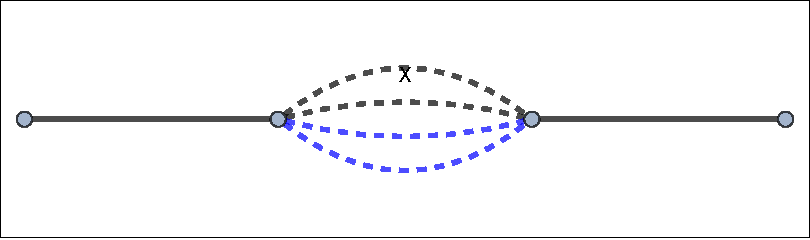
\includegraphics[width=0.6\linewidth]{img/1ma9r62jq7ebq.pdf}
\end{figure}

We can style a fully massive 1-loop box in a very creative way

\begin{Shaded}
\begin{Highlighting}[]
\NormalTok{FCLoopIntegralToGraph}\OperatorTok{[}\NormalTok{FAD}\OperatorTok{[\{}\FunctionTok{p}\OperatorTok{,}\NormalTok{ m1}\OperatorTok{\},} \OperatorTok{\{}\FunctionTok{p} \SpecialCharTok{+}\NormalTok{ q1}\OperatorTok{,}\NormalTok{ m2}\OperatorTok{\},} \OperatorTok{\{}\FunctionTok{p} \SpecialCharTok{+}\NormalTok{ q1 }\SpecialCharTok{+}\NormalTok{ q2}\OperatorTok{,}\NormalTok{ m3}\OperatorTok{\},} \OperatorTok{\{}\FunctionTok{p} \SpecialCharTok{+}\NormalTok{ q1 }\SpecialCharTok{+}\NormalTok{ q2 }\SpecialCharTok{+}\NormalTok{ q3}\OperatorTok{,}\NormalTok{ m4}\OperatorTok{\}],} \OperatorTok{\{}\FunctionTok{p}\OperatorTok{\}]}
\NormalTok{FCLoopGraphPlot}\OperatorTok{[}\SpecialCharTok{\%}\OperatorTok{,} \FunctionTok{GraphPlot} \OtherTok{{-}\textgreater{}} \OperatorTok{\{}\FunctionTok{MultiedgeStyle} \OtherTok{{-}\textgreater{}} \FloatTok{0.35}\OperatorTok{,} \FunctionTok{Frame} \OtherTok{{-}\textgreater{}} \ConstantTok{True}\OperatorTok{\},} \FunctionTok{Style} \OtherTok{{-}\textgreater{}} \OperatorTok{\{}
    \OperatorTok{\{}\StringTok{"InternalLine"}\OperatorTok{,}\NormalTok{ \_}\OperatorTok{,}\NormalTok{ \_}\OperatorTok{,} \AttributeTok{mm\_} \SpecialCharTok{/}\NormalTok{; ! }\FunctionTok{FreeQ}\OperatorTok{[}\NormalTok{mm}\OperatorTok{,}\NormalTok{ m1}\OperatorTok{]\}} \OtherTok{{-}\textgreater{}} \OperatorTok{\{}\FunctionTok{Red}\OperatorTok{,} \FunctionTok{Thick}\OperatorTok{\},} 
    \OperatorTok{\{}\StringTok{"InternalLine"}\OperatorTok{,}\NormalTok{ \_}\OperatorTok{,}\NormalTok{ \_}\OperatorTok{,} \AttributeTok{mm\_} \SpecialCharTok{/}\NormalTok{; ! }\FunctionTok{FreeQ}\OperatorTok{[}\NormalTok{mm}\OperatorTok{,}\NormalTok{ m2}\OperatorTok{]\}} \OtherTok{{-}\textgreater{}} \OperatorTok{\{}\FunctionTok{Blue}\OperatorTok{,} \FunctionTok{Thick}\OperatorTok{\},} 
    \OperatorTok{\{}\StringTok{"InternalLine"}\OperatorTok{,}\NormalTok{ \_}\OperatorTok{,}\NormalTok{ \_}\OperatorTok{,} \AttributeTok{mm\_} \SpecialCharTok{/}\NormalTok{; ! }\FunctionTok{FreeQ}\OperatorTok{[}\NormalTok{mm}\OperatorTok{,}\NormalTok{ m3}\OperatorTok{]\}} \OtherTok{{-}\textgreater{}} \OperatorTok{\{}\FunctionTok{Green}\OperatorTok{,} \FunctionTok{Thick}\OperatorTok{\},} 
    \OperatorTok{\{}\StringTok{"InternalLine"}\OperatorTok{,}\NormalTok{ \_}\OperatorTok{,}\NormalTok{ \_}\OperatorTok{,} \AttributeTok{mm\_} \SpecialCharTok{/}\NormalTok{; ! }\FunctionTok{FreeQ}\OperatorTok{[}\NormalTok{mm}\OperatorTok{,}\NormalTok{ m4}\OperatorTok{]\}} \OtherTok{{-}\textgreater{}} \OperatorTok{\{}\FunctionTok{Purple}\OperatorTok{,} \FunctionTok{Thick}\OperatorTok{\},}
    \OperatorTok{\{}\StringTok{"ExternalLine"}\OperatorTok{,}\NormalTok{ q1}\OperatorTok{\}} \OtherTok{{-}\textgreater{}} \OperatorTok{\{}\FunctionTok{Brown}\OperatorTok{,} \FunctionTok{Thick}\OperatorTok{,} \FunctionTok{Dashed}\OperatorTok{\}} 
   \OperatorTok{\}]}
\end{Highlighting}
\end{Shaded}

\begin{dmath*}\breakingcomma
\left\{\{-4\to 4,-3\to 1,-2\to 2,-1\to 3,1\to 2,1\to 4,2\to 3,3\to 4\},\left\{\text{q1}-\text{q2}-\text{q3},\text{q1},\text{q2},\text{q3},\left\{p+\text{q1}+\text{q2},1,-\text{m3}^2\right\},\left\{p+\text{q1}+\text{q2}+\text{q3},1,-\text{m4}^2\right\},\left\{p+\text{q1},1,-\text{m2}^2\right\},\left\{p,1,-\text{m1}^2\right\}\right\},\left\{0,0,0,0,\frac{1}{(p^2-\text{m1}^2+i \eta )},\frac{1}{((p+\text{q1})^2-\text{m2}^2+i \eta )},\frac{1}{((p+\text{q1}+\text{q2})^2-\text{m3}^2+i \eta )},\frac{1}{((p+\text{q1}+\text{q2}+\text{q3})^2-\text{m4}^2+i \eta )}\right\},1\right\}
\end{dmath*}

\begin{figure}[!ht]
\centering
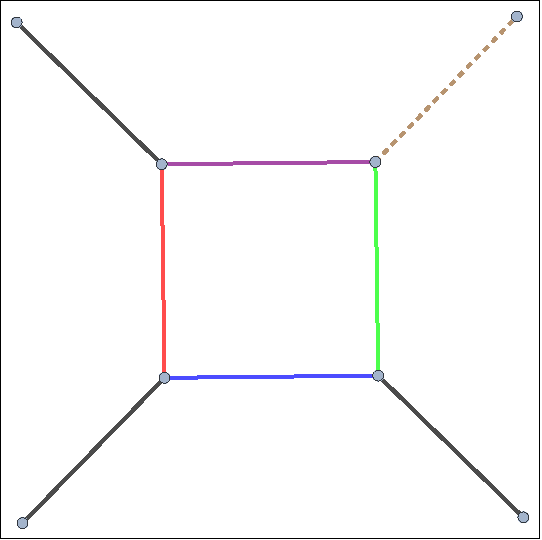
\includegraphics[width=0.6\linewidth]{img/02dm2nagbs2f8.pdf}
\end{figure}

The same goes for a 2-loop box with 3 massive lines

\begin{Shaded}
\begin{Highlighting}[]
\NormalTok{FCLoopIntegralToGraph}\OperatorTok{[}\NormalTok{FAD}\OperatorTok{[\{}\NormalTok{p1}\OperatorTok{,}\NormalTok{ m1}\OperatorTok{\},} \OperatorTok{\{}\NormalTok{p2}\OperatorTok{,}\NormalTok{ m2}\OperatorTok{\},} \OperatorTok{\{}\NormalTok{Q1 }\SpecialCharTok{+}\NormalTok{ p1}\OperatorTok{,}\NormalTok{ m3}\OperatorTok{\},}\NormalTok{ Q2 }\SpecialCharTok{{-}}\NormalTok{ p1}\OperatorTok{,}\NormalTok{ Q1 }\SpecialCharTok{+}\NormalTok{ p1 }\SpecialCharTok{+}\NormalTok{ p2}\OperatorTok{,}\NormalTok{ Q2 }\SpecialCharTok{{-}}\NormalTok{ p1 }\SpecialCharTok{{-}}\NormalTok{ p2}\OperatorTok{,} 
\NormalTok{    Q2 }\SpecialCharTok{+}\NormalTok{ Q3 }\SpecialCharTok{{-}}\NormalTok{ p1 }\SpecialCharTok{{-}}\NormalTok{ p2}\OperatorTok{],} \OperatorTok{\{}\NormalTok{p1}\OperatorTok{,}\NormalTok{ p2}\OperatorTok{\}]} 
 
\NormalTok{FCLoopGraphPlot}\OperatorTok{[}\SpecialCharTok{\%}\OperatorTok{,} \FunctionTok{GraphPlot} \OtherTok{{-}\textgreater{}} \OperatorTok{\{}\FunctionTok{MultiedgeStyle} \OtherTok{{-}\textgreater{}} \FloatTok{0.35}\OperatorTok{,} \FunctionTok{Frame} \OtherTok{{-}\textgreater{}} \ConstantTok{True}\OperatorTok{\},} \FunctionTok{Style} \OtherTok{{-}\textgreater{}} \OperatorTok{\{}
    \OperatorTok{\{}\StringTok{"InternalLine"}\OperatorTok{,}\NormalTok{ \_}\OperatorTok{,}\NormalTok{ \_}\OperatorTok{,} \AttributeTok{mm\_} \SpecialCharTok{/}\NormalTok{; ! }\FunctionTok{FreeQ}\OperatorTok{[}\NormalTok{mm}\OperatorTok{,}\NormalTok{ m1}\OperatorTok{]\}} \OtherTok{{-}\textgreater{}} \OperatorTok{\{}\FunctionTok{Red}\OperatorTok{,} \FunctionTok{Thick}\OperatorTok{\},} 
    \OperatorTok{\{}\StringTok{"InternalLine"}\OperatorTok{,}\NormalTok{ \_}\OperatorTok{,}\NormalTok{ \_}\OperatorTok{,} \AttributeTok{mm\_} \SpecialCharTok{/}\NormalTok{; ! }\FunctionTok{FreeQ}\OperatorTok{[}\NormalTok{mm}\OperatorTok{,}\NormalTok{ m2}\OperatorTok{]\}} \OtherTok{{-}\textgreater{}} \OperatorTok{\{}\FunctionTok{Blue}\OperatorTok{,} \FunctionTok{Thick}\OperatorTok{\},} 
    \OperatorTok{\{}\StringTok{"InternalLine"}\OperatorTok{,}\NormalTok{ \_}\OperatorTok{,}\NormalTok{ \_}\OperatorTok{,} \AttributeTok{mm\_} \SpecialCharTok{/}\NormalTok{; ! }\FunctionTok{FreeQ}\OperatorTok{[}\NormalTok{mm}\OperatorTok{,}\NormalTok{ m3}\OperatorTok{]\}} \OtherTok{{-}\textgreater{}} \OperatorTok{\{}\FunctionTok{Green}\OperatorTok{,} \FunctionTok{Thick}\OperatorTok{\},} 
    \OperatorTok{\{}\StringTok{"InternalLine"}\OperatorTok{,}\NormalTok{ \_}\OperatorTok{,}\NormalTok{ \_}\OperatorTok{,} \AttributeTok{mm\_} \SpecialCharTok{/}\NormalTok{; ! }\FunctionTok{FreeQ}\OperatorTok{[}\NormalTok{mm}\OperatorTok{,}\NormalTok{ m4}\OperatorTok{]\}} \OtherTok{{-}\textgreater{}} \OperatorTok{\{}\FunctionTok{Purple}\OperatorTok{,} \FunctionTok{Thick}\OperatorTok{\},}
    \OperatorTok{\{}\StringTok{"ExternalLine"}\OperatorTok{,}\NormalTok{ q1}\OperatorTok{\}} \OtherTok{{-}\textgreater{}} \OperatorTok{\{}\FunctionTok{Brown}\OperatorTok{,} \FunctionTok{Thick}\OperatorTok{,} \FunctionTok{Dashed}\OperatorTok{\}} 
   \OperatorTok{\}]}
\end{Highlighting}
\end{Shaded}

\begin{dmath*}\breakingcomma
\left\{\{-4\to 4,-3\to 1,-2\to 2,-1\to 3,1\to 4,1\to 6,2\to 3,2\to 6,3\to 5,4\to 5,5\to 6\},\left\{\text{Q1}-\text{Q2}-\text{Q3},\text{Q1},\text{Q2},\text{Q3},\{-\text{p1}-\text{p2}+\text{Q2}+\text{Q3},1,0\},\{-\text{p1}-\text{p2}+\text{Q2},1,0\},\left\{\text{p1},1,-\text{m1}^2\right\},\{\text{Q2}-\text{p1},1,0\},\left\{\text{p1}+\text{Q1},1,-\text{m3}^2\right\},\{\text{p1}+\text{p2}+\text{Q1},1,0\},\left\{\text{p2},1,-\text{m2}^2\right\}\right\},\left\{0,0,0,0,\frac{1}{((\text{p1}+\text{p2}+\text{Q1})^2+i \eta )},\frac{1}{((\text{Q2}-\text{p1})^2+i \eta )},\frac{1}{(\text{p2}^2-\text{m2}^2+i \eta )},\frac{1}{(\text{p1}^2-\text{m1}^2+i \eta )},\frac{1}{((\text{p1}+\text{Q1})^2-\text{m3}^2+i \eta )},\frac{1}{((-\text{p1}-\text{p2}+\text{Q2})^2+i \eta )},\frac{1}{((-\text{p1}-\text{p2}+\text{Q2}+\text{Q3})^2+i \eta )}\right\},1\right\}
\end{dmath*}

\begin{figure}[!ht]
\centering
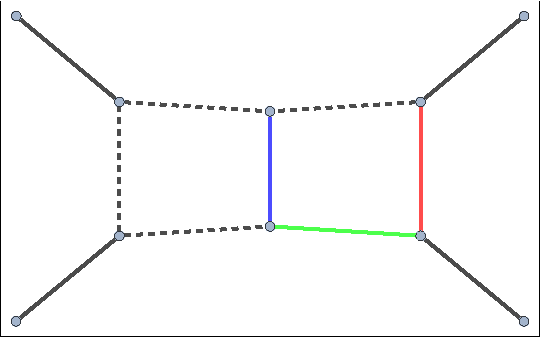
\includegraphics[width=0.6\linewidth]{img/08mmgiizwltpy.pdf}
\end{figure}

One can also (sort of) visualize the momentum flow, where we use powers
to denote the dots

\begin{Shaded}
\begin{Highlighting}[]
\NormalTok{FCLoopIntegralToGraph}\OperatorTok{[}\NormalTok{FCTopology}\OperatorTok{[}\NormalTok{topo1X1}\OperatorTok{,} \OperatorTok{\{}\NormalTok{SFAD}\OperatorTok{[\{\{}\NormalTok{p2}\OperatorTok{,} \DecValTok{0}\OperatorTok{\},} \OperatorTok{\{}\NormalTok{m1}\SpecialCharTok{\^{}}\DecValTok{2}\OperatorTok{,} \DecValTok{1}\OperatorTok{\},} \DecValTok{2}\OperatorTok{\}],} 
\NormalTok{     SFAD}\OperatorTok{[\{\{}\NormalTok{p1}\OperatorTok{,} \DecValTok{0}\OperatorTok{\},} \OperatorTok{\{}\NormalTok{m1}\SpecialCharTok{\^{}}\DecValTok{2}\OperatorTok{,} \DecValTok{1}\OperatorTok{\},} \DecValTok{2}\OperatorTok{\}],} 
\NormalTok{     SFAD}\OperatorTok{[\{\{}\NormalTok{p2 }\SpecialCharTok{+}\NormalTok{ p3}\OperatorTok{,} \DecValTok{0}\OperatorTok{\},} \OperatorTok{\{}\DecValTok{0}\OperatorTok{,} \DecValTok{1}\OperatorTok{\},} \DecValTok{1}\OperatorTok{\}],}\NormalTok{ SFAD}\OperatorTok{[\{\{}\NormalTok{p2 }\SpecialCharTok{+}\NormalTok{ p3}\OperatorTok{,} \DecValTok{0}\OperatorTok{\},} \OperatorTok{\{}\DecValTok{0}\OperatorTok{,} \DecValTok{1}\OperatorTok{\},} \DecValTok{1}\OperatorTok{\}],}
\NormalTok{     SFAD}\OperatorTok{[\{\{}\NormalTok{p1 }\SpecialCharTok{+}\NormalTok{ p3}\OperatorTok{,} \DecValTok{0}\OperatorTok{\},} \OperatorTok{\{}\DecValTok{0}\OperatorTok{,} \DecValTok{1}\OperatorTok{\},} \DecValTok{1}\OperatorTok{\}],}\NormalTok{ SFAD}\OperatorTok{[\{\{}\NormalTok{p1 }\SpecialCharTok{+}\NormalTok{ p2 }\SpecialCharTok{+}\NormalTok{ p3}\OperatorTok{,} \DecValTok{0}\OperatorTok{\},} \OperatorTok{\{}\DecValTok{0}\OperatorTok{,} \DecValTok{1}\OperatorTok{\},} \DecValTok{1}\OperatorTok{\}]\},} \OperatorTok{\{}\NormalTok{p1}\OperatorTok{,}\NormalTok{ p2}\OperatorTok{,}\NormalTok{ p3}\OperatorTok{\},} \OperatorTok{\{\},} \OperatorTok{\{\},} \OperatorTok{\{\}]]} 
 
\NormalTok{FCLoopGraphPlot}\OperatorTok{[}\SpecialCharTok{\%}\OperatorTok{,} \FunctionTok{GraphPlot} \OtherTok{{-}\textgreater{}} \OperatorTok{\{}\FunctionTok{MultiedgeStyle} \OtherTok{{-}\textgreater{}} \FloatTok{0.35}\OperatorTok{,} \FunctionTok{Frame} \OtherTok{{-}\textgreater{}} \ConstantTok{True}\OperatorTok{\},} \FunctionTok{Labeled} \OtherTok{{-}\textgreater{}} \OperatorTok{\{}
    \OperatorTok{\{}\StringTok{"InternalLine"}\OperatorTok{,} \AttributeTok{x\_}\OperatorTok{,} \AttributeTok{pow\_}\OperatorTok{,}\NormalTok{ \_}\OperatorTok{\}}\NormalTok{ :\textgreater{} }\FunctionTok{x}\SpecialCharTok{\^{}}\NormalTok{pow}\OperatorTok{,} 
    \OperatorTok{\{}\StringTok{"ExternalLine"}\OperatorTok{,}\NormalTok{ \_}\OperatorTok{\}}\NormalTok{ :\textgreater{} }\OperatorTok{\{\}\}]}
\end{Highlighting}
\end{Shaded}

\begin{dmath*}\breakingcomma
\left\{\{1\to 2,1\to 3,1\to 3,2\to 3,2\to 3\},\left(
\begin{array}{ccc}
 \;\text{p1}+\text{p2}+\text{p3} & 1 & 0 \\
 \;\text{p1}+\text{p3} & 1 & 0 \\
 \;\text{p2} & 2 & -\text{m1}^2 \\
 \;\text{p2}+\text{p3} & 2 & 0 \\
 \;\text{p1} & 2 & -\text{m1}^2 \\
\end{array}
\right),\left\{\frac{1}{((\text{p1}+\text{p3})^2+i \eta )},\frac{1}{((\text{p2}+\text{p3})^2+i \eta )},\frac{1}{((\text{p1}+\text{p2}+\text{p3})^2+i \eta )},\frac{1}{(\text{p1}^2-\text{m1}^2+i \eta )},\frac{1}{(\text{p2}^2-\text{m1}^2+i \eta )}\right\},1\right\}
\end{dmath*}

\begin{figure}[!ht]
\centering
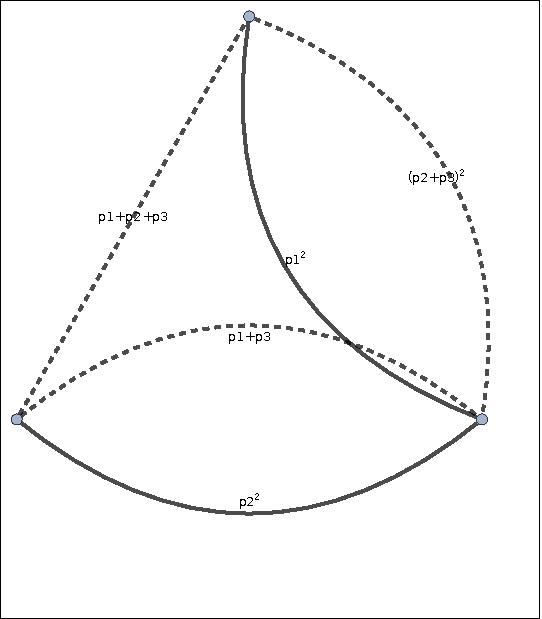
\includegraphics[width=0.6\linewidth]{img/12ux83if2wffb.pdf}
\end{figure}
\end{document}
